\documentclass[10pt,journal]{IEEEtran}  %10pt, sans, memo

\usepackage{amsthm}

\usepackage[utf8]{inputenc}

\usepackage{tikz}
\usepackage{tikzscale}
\usepackage{pgfplots}

\usepackage{subcaption}

\usepackage{booktabs}
\usepackage{graphicx}
\usepackage{mathtools}
\usepackage{breqn}
\usepackage[noadjust]{cite}
\usepackage{hyperref}
\usepackage{cleveref}

\bibliographystyle{IEEEtran}

\author{Jonathan Dyer}
\date{\today}
\title{Imaging Trends and the Future of \\High Resolution Satellite Remote Sensing}
\hypersetup{
 pdfauthor={Jonathan Dyer},
 pdftitle={EO Modalities},
 pdfkeywords={},
 pdfsubject={},
 pdfcreator={}, 
 pdflang={English}}

\newcommand{\includefigure}[3]
{
  \begin{figure}[h!]
  \centering
  \includegraphics{#1}
  \caption[]{#3}
  \label{#2}
  \end{figure}
}
\DeclarePairedDelimiter{\abs}{\lvert}{\rvert}
\DeclarePairedDelimiter{\norm}{\lVert}{\rVert}

% Don't allow these words to by broken (hyphenated) across lines/pages
\hyphenation{NIIRS}
%\hyphenation{GIQE-5}

\begin{document}

\newtheorem{mydef}{Definition}
\newtheorem{observation}{Observation}

\makeatletter
\newcommand\footnoteref[1]{\protected@xdef\@thefnmark{\ref{#1}}\@footnotemark}
\makeatother

\author{Jonathan~Dyer\IEEEauthorrefmark{1}\thanks{\IEEEauthorrefmark{1}Former~Chief~Engineer, Skybox~Imaging,~Terra~ Bella},~\IEEEmembership{Member,~IEEE,}
        Paul~Boerner\IEEEauthorrefmark{2}\thanks{\IEEEauthorrefmark{2}Imaging Systems Engineer, Planet, Inc.},~\IEEEmembership{Member,~IEEE}
        and~Mark~Robertson\IEEEauthorrefmark{3}\thanks{\IEEEauthorrefmark{3}Former Lead Image Processing, Skybox Imaging, Terra Bella}%
}

\markboth{IEEE Transactions on Geoscience and Remote Sensing}%
{}
        
        
\IEEEtitleabstractindextext{%
\begin{abstract}
Many of the technology and investment trends that ushered in the so-called ``SmallSat Revolution'' will continue or accelerate but there is a paucity of analysis available in the open literature regarding the system design implications of these trends.  While these systems may not replace more traditional remote sensing systems in the near term, in many cases they are highly complementary such that interest and investment will continue to grow.

The authors identify the trends in imaging and micro-electronics driven by investments in such applications as smart phones and 4k TV and analyze the impact the associated technologies can have in new remote sensing spacecraft.  The commercially-driven technologies present large opportunities for cost reduction and performance improvements but require new system architectures and approaches.
\end{abstract}

% Note that keywords are not normally used for peerreview papers.
\begin{IEEEkeywords}
IEEE, Remote Sensing, Satellite, Imaging, Image resolution, CMOS Integrated Circuits, Systems Engineering.
\end{IEEEkeywords}}

% make the title area
\maketitle

\IEEEdisplaynontitleabstractindextext

\tableofcontents

\section{Introduction}
\label{sec:introduction}

The last 15 years have seen a massive upheaval in digital imaging culminating in almost total obsolescence of film-based imaging.  Initially driven by the pro-sumer DSLR and pocket camera market, the trend has continued and accelerated with the introduction and refinement of high quality cameras in to smart phones and the digitization of the TV and movie industries.

Satellite remote sensing systems underwent a similar revolution roughly 40 years earlier as film-based systems were phased out in favor of CCD-based electronic line scanners.  While the specific demanding requirements of satellite remote sensing drove much of the early technology investment and development in digital electronic imaging, far more investment is now being applied in the commercial arena than in further refinement of now mature CCD-based line scan sensors.

We believe that the future of the satellite remote-sensing industry will be in leveraging the massive investment in commercial digital and computational imaging technologies rather than continued large-scale investment in standalone technologies for these systems and that this shift presents both opportunities and challenges to new systems.

\section{Trends}
In order to motivate the subsequent discussion, we identify and discuss the ``SmallSat'' philosophical trend and two technology trends uniquely enabling it in remote sensing systems.

\subsection{Trend to Smaller Spacecraft}

\label{sec:smallsat}
There is a large and growing interest in what can be accomplished with much smaller spacecraft.  This trend is driven by 
\begin{itemize}
    \item Reduced appetite for the large and ballooning costs of traditional systems
    \item Recognition of the mission level advantages offered by constellations of satellites (homogeneous or with sensor disaggregation) enabled by lower cost systems
    \item Demonstration of high-performance remote sensing SmallSats developed at low cost by small, commercially funded teams
\end{itemize} 

There is significant evidence indicating that mission cost is non-linearly correlated with spacecraft size and complexity.  Indeed \cite{bearden} has shown with high correlation that 
\begin{equation*}
    C \sim m^{1.261},
\end{equation*}
implying cost $C$ is super-linearly impacted by mass, $m$.  Because for spacecraft systems $m \sim \chi^n$ where $\chi$ is a characteristic spacecraft dimension and $n$ is typically between 2 and 3, we can also say
\begin{equation}
C \sim \chi^{3+}
\end{equation}

Similar arguments can be derived from other cost scaling observations such as Meinel's Law \cite{meinel} for telescopes which states
\begin{equation}
    C \sim D_{ap}^{2.7},
\end{equation}
where $D_{ap}$ is aperture diameter.

This polynomial relationship between size and cost indicates that there are significant savings available in shrinking system size down subject, of course to fundamental physical limits such as diffraction-limited resolution.  

\subsection{Sensor Technology}
\label{sec:sensor_trends}

Historically, space-based remote sensing systems have utilized CCD-based Time Delayed Integration (TDI) line-scan sensors.  Modern TDI sensors are a mature technology with several very desirable characteristics for high resolution remote sensing:

\begin{itemize}
    \item Mechanism-free relative motion compensation through charge transfer
    \item High quantum efficiency and fill fractions
    \item Low noise
    \item Relatively high readout line-rates compatible with needs of high resolution systems
    \item Reasonable radiation tolerance
\end{itemize}

However the unique requirements associated with space-based sensors implies that the sensors are niche, low volume and typically very expensive to develop, integrate and use.

Meanwhile the large commercial investment in imaging sensors driven by the consumer photography/cinema, machine vision and smart phone industries has resulted in incredibly high performance image sensors available at high volume and low cost.  The big trends that have developed due to this investment are:

\begin{itemize}
    \item Movement from CCD to CMOS detector technology
    \item Drive to smaller pixels to enable compact cameras \cite{isscc2016}
    \item Significant increase in detector read-out rates at low noise
\end{itemize}

% \begin{figure}[h!]
% 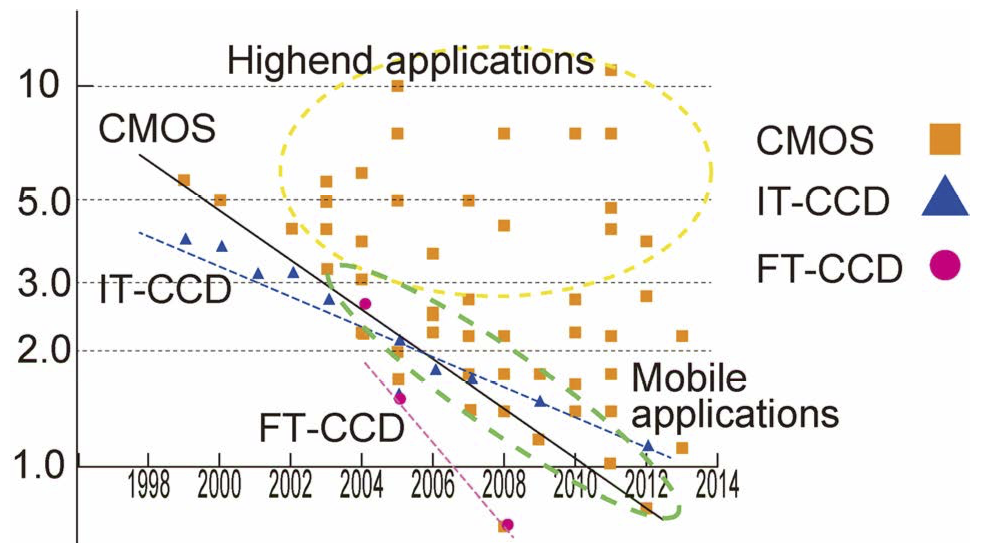
\includegraphics[width=0.45\textwidth]{figures/pixel_trend.png}
% \caption[]{Trends in commercial sensor pixel sizes from \cite{isscc2016}.  Note the ordinate is in units of microns}
% \label{fig:pix_trend}
% \end{figure}

CCD-based sensors still hold some performance advantages over CMOS sensors, but the capability gap has narrowed almost entirely. The manufacturing and read-out rate advantages offered by CMOS have led to its wholesale adoption in the consumer / commercial world.

When developing new remote sensing systems, the capabilities of modern commercial detectors promise the potential of smaller, less expensive systems with similar or better imaging performance to traditional TDI CCD-based systems.  However to realize this promise, the imaging system designer must consider the unique capabilities and shortcomings of the technology.

\subsection{Non-Imaging Commercial Electronic Trends}

In addition to the rapid advances in commercial imaging technology, Moore's law has continued to drive massive increase in microelectronic integration density with the associated performance, cost and device size improvements.

Indeed in recent years much of the emphasis has been in large-scale functional integration into single die ``system-on-chip'' (SoC) devices that operate at very high performance/watt for the consumer devices industry.  Such devices are uniquely enabling for small spacecraft in that, just as with consumer devices, they enable massive functionality in a small, low power package and limit the amount of functional engineering ``glue'' required, shortening design cycles.  Stated more directly, the computational power most people have in their pockets today was unavailable in large, complex spacecraft ten years ago.

Similar arguments can be made for:

\begin{itemize}
    \item High density solid-state storage (Flash memory)
    \item Dedicated signal- and image-processing hardware for compression or computational imaging
    \item Digital modulation and radio technologies
    \item Inertial sensors
\end{itemize}

Indeed, one can look at many of our personal consumer electronic devices and see the applicability to spacecraft in virtually every technology.  And these technologies have investment rates orders-of-magnitude higher than dedicated aerospace technologies.

Historically there has been resistance to the utilization of commercial electronics technologies for space applications due to reliability concerns, both intrinsic and due to the space environment.  Again, several developments make such resistance less defensible:

\begin{itemize}
    \item Demonstration of high uptime and reliable operation of COTS-based avionics in LEO \cite{careful_cots}.
    \item High demonstrated statistical reliability of commercially available components qualified to operate over thermal ranges much more severe than typical in-space environments, e.g. auto, industrial.
    \item Substantial improvement in CMOS latch-up susceptibility
    \item Pervasive integration of hardware single-event protection driven by sea-level single-event susceptibility of modern high integration devices
\end{itemize}

For small systems these trends are uniquely empowering and are more easily adoptable with lower cost (and hence less risk-averse) systems.  

Furthermore the ability to incorporate high performance compute, storage and communications in space- and power-constrained systems invalidates some of the long-held constraints on other spacecraft systems such as the ability to perform near-real-time on-board image processing.

\section{Remote Sensing Metrics}
\label{sec:Metrics}
In order to compare different remote sensing systems, we need quantitative metrics.  The metrics we will introduce are fundamentally related to the data produced by such systems and are in two categories - \emph{quality} and \emph{volume}.  In a value-based assessment, quality and volume would form the numerator of a global value metric with cost in the denominator.

\subsection{Image Quality}
\label{sec:iq}

Image quality is a complex, multi-faceted subject and while there is no perfect model or metric, substantial work has gone into quantifying the image quality of high resolution remote sensing systems.  Before jumping into integrated image quality models, we will define the geometric and radiometric components of image quality.

\subsubsection{Resolution, NIIRS and GIQE}
Resolution is a key component of image quality but is a surprisingly difficult-to-define metric.  Often Ground Sample Distance, $GSD$ is used as a proxy for resolution under the assumption of near-critical sampling.
Alternatively, Ground Resolution Distance, $GRD$, is used where $GRD$ is a form of the diffraction-limited optical resolution such that given by the Rayleigh Criterion:
\begin{equation}
    GRD = 1.22 \frac{\lambda R}{D_{ap}},
\end{equation}

where $R$ is range to target (spacecraft altitude if Nadir-pointed),  $D_{ap}$ is the aperture diameter and $\lambda$ is the weighted center-wavelength of the sanpled spectral band.

Comparing image quality purely on $GSD$ or $GRD$ becomes problematic for systems with varying $Q$ and/or $SNR$ (see Section~\ref{sec:q}) because depending on the sampling or SNR regimes resolvability may first be constrained by sampling, diffraction or SNR.  Figures~\ref{fig:snr_mtf_q1}, \ref{fig:snr_mtf_q2} illustrate this graphically.

\includefigure{figures/SNR_mtf_Q1.pdf}{fig:snr_mtf_q1}{Image demonstrating the impact of SNR and MTF (diffraction / blur) on resolve-ability for $Q=1$.  Note red-dotted line indicates the sampling frequency.}

\includefigure{figures/SNR_mtf_Q2.pdf}{fig:snr_mtf_q2}{Image demonstrating the impact of SNR and MTF (diffraction / blur) on resolve-ability for $Q=2$  Note red-dotted line indicates the sampling frequency.}

More holistic image quality formulations typically refer back to \emph{resolvability} or the ability to distinguish objects or features of a given size in an image.

High resolution space-based systems are typically evaluated by quantitative ``image interpretability'' scales, the best known being the National Image Interpretability Rating Scale, or NIIRS.

NIIRS rating is described by specific scene intepretation standards, examples of which are shown in Table~\ref{table:NIIRS}\cite{niirs}.

\begin{table}[h!t]
\resizebox{.45\textwidth}{!}{%
\begin{tabular}{@{}lll@{}}
\toprule
\textbf{NIIRS} & \textbf{GRD}          & \textbf{Description}                                                                                                                             \\ \toprule
3     & 2.5m - 4.5m  & \begin{tabular}[c]{@{}l@{}}Identify a road as divided or undivided\\ Detect rows of automobiles in a parking lot\end{tabular}           \\ \midrule
4    & 1.2m - 2.5m  & \begin{tabular}[c]{@{}l@{}}Detect barriers/obstacles (barrels) on runways\\ Distinguish between locomotives and railcars\end{tabular}   \\ \midrule
5     & 0.75m - 1.2m & \begin{tabular}[c]{@{}l@{}}Identify individual lines painted on paved roads,  parking lots\\ Identify fallen utility poles\end{tabular} \\ \midrule
6     & 0.4m - 0.75m & \begin{tabular}[c]{@{}l@{}}Detect individuals, when not in a group\\ Detect small road signs in an urban area\end{tabular}              \\ \bottomrule
\end{tabular}%
}
\centering
\caption{NIIRS definitions}
\label{table:NIIRS}
\end{table}

NIIRS is a logarithmic scale traditionally evaluated by trained human image interpreters.  However, much work has gone into developing semi-analytic regressions to predict NIIRS from basic image quality parameters such as sharpness, signal-to-noise ratio (SNR), etc. The Generalized Image Quality Equation (GIQE) is an example of such a function; we will use the 5th version, GIQE-5 which is defined in eq. \eqref{eq:giqe5}.

\begin{dmath}
NIIRS = 4.4 - 3.32 \log(GSD_{m}) + 3.32 \left[1 - e^{\frac{-5.308}{\Delta SNR}}\right]\log(RER_0)
- 0.402 \log(RER_0)^4 - 2.92/\Delta SNR - 0.069N_{smear},
\label{eq:giqe5}
\end{dmath}
where $GSD_{m}$\footnote{GSD units must be paid close attention to -- many references list GIQE using units of inches for GSD.  In this case, the first parameter in the equation is 9.7 rather than 4.4 because $4.4 - 3.32\log{\left(39.4 \frac{in}{m}\right)} \approx 9.7$} is the ground sample distance in meters, $\Delta SNR$ is difference between $SNR$ for a 15\% and 8\% target reflectance, $RER_0$ is the raw Relative Edge Response (without sharpening or MTFC) and $N_{smear}$ is the number of pixels of linear smear.

GIQE-5 is fairly well validated again human interpreters~\cite{giqe5} and nicely captures the trade-off between various imaging system parameters such as $SNR$ and $GSD$.  Note that GIQE-5 is logarithmic in resolution such that a halving of $GSD$ (proportional to resolution when holding other parameters constant) results in a NIIRS improvement of 1.

Based on this definition, one can use GIQE-5 to define an effective ground resolvability distance $GRD_{eff}$
\begin{equation}
    GRD_{eff}(m) = 10^{\frac{4.4 - NIIRS}{3.32}}.
    \label{eq:grd_eff}
\end{equation}

% \cite{auelmann_iq} shows that:

% \begin{equation}
%     GRD = \frac{R\times IFOV}{RER} = \frac{R\lambda_{mean}}{D_{ap} Q \times RER (Q)}
% \label{eq:alpha_eff}
% \end{equation}

% and that a good approximation for the GIQE-based $GRD$ for diffraction limited systems is given by:

% \begin{equation}
%     GRD \approx \frac{R\lambda_{mean}}{D_{ap}}\left[1 + \frac{1}{Q^{1.35}}\right]^{1/1.35}
% \label{eq:alpha_eff_approx}
% \end{equation}

\includefigure{figures/resolution_q.pgf}{fig:resolution_q}{Relationship of GRD and GSD as resolution metrics as a function of Q}

Notice in Figure~\ref{fig:resolution_q} that GRD asymptotes at $Q=2$ due to diffraction but that GSD continues decreasing monotonically.  This is because optical systems do not pass spatial frequency beyond the diffraction limit which is critically sampled at $Q=2$.

\subsubsection{Dynamic Range ($DR$) and Signal-to-Noise Ratio ($SNR$)}

Dynamic range and signal-to-noise ratio are closely related by subtly different measures of radiometric performance.

Dynamic range is defined as the ratio of maximum-to-minimum signal level that the system can capture or represent in an image

\begin{equation*}
    DR = \frac{s_{max}}{s_{min}}.
\end{equation*}

The minimum signal level is the noise-floor of the system, $s_{min} = \sigma$ where $\sigma$ represents all non-signal-correlated noise sources in the system including read noise, dark current, quantization, etc.

The maximum signal is the maximum number of photo-electrons the system can capture for one output image pixel and is limited by the well depth of a pixel, $s_{max} = N_{e^-}^{FWC}$ for single-exposure systems.  Note that in digitally oversampled systems (covered later), the digital oversampling factor directly expands dynamic range by increasing the effective well depth such that $s_{max} = N_s N_{e^-}^{FWC}$ where $N_s$ is the oversampling ratio


\begin{equation}
    N_s = \text{floor}\left(\frac{GSD \times LR}{V_{gnd}}\right)
    \label{eq:N_s}
\end{equation}

where $LR$ is the time-rate that lines (rows) are read from the detector in lines/second.

Oversampling also affects $s_{min}$ and it can be shown that, for equally exposed samples

\begin{equation}
    DR = \sqrt{N_s}\frac{N_{e^-}^{FWC}}{\sigma_{uncor}}.
\label{eq:DR_OS}
\end{equation}

Dynamic range is a very important quality parameter for remote sensing systems because the dynamic range of terrestrial natural scenes can be quite high. 

\begin{figure}[h!]
\centering
\begin{subfigure}{0.31\linewidth}
\centering
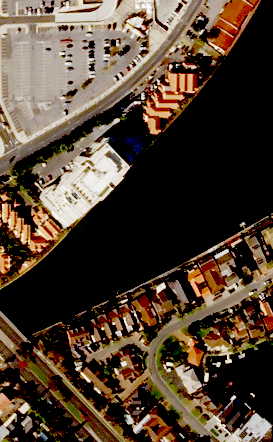
\includegraphics[width = \textwidth]{figures/pb_bad_dr_low.png}
\end{subfigure}
\begin{subfigure}{0.31\linewidth}
\centering
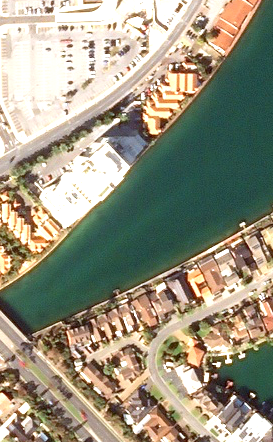
\includegraphics[width = \textwidth]{figures/pb_bad_dr_high.png}
\end{subfigure}
\begin{subfigure}{0.31\linewidth}
\centering
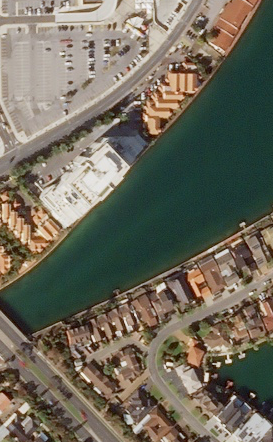
\includegraphics[width = \textwidth]{figures/pb_good_dr.png}
\end{subfigure}
\caption{The first two images have relatively low dynamic range.  The first is under-exposed and the second over-.  Note the details lost in shadows in the first and highlights (parking lot) in the second when compared with the third image which has about 90dB of DR}
\end{figure}

For systems that digitally oversample with unequal exposures, the dynamic range can be even larger as is shown in Section~\ref{sec:hdr}.
Signal-to-noise ratio, $SNR$, like dynamic range depends critically on both the detector well depth and its noise characteristics.  However signal-to-noise ratio is not purely a system-defined metric but depends also on the scene being imaged and as well as exposure parameters.  $SNR$ is defined as

\begin{equation*}
    SNR = \frac{s}{\sigma_{noise}}.
\end{equation*}

The noise, $\sigma_{noise}$ consists of the same sources discussed for $DR$ but also the shot-noise associated with the signal, $s$.  Because arrival rate of incoming photons obey Poisson statistics, it can be shown that $\sigma_{shot} = \sqrt{s}$ such that

\begin{equation*}
    SNR = \frac{s}{\sqrt{\sum{\sigma_i^2} + s}}.
\end{equation*}

In order to state an $SNR$, the signal, $s$, must be constrained by other system parameters and some exposure.  Typically $SNR$ is specified with respect to a specific target reflectance or top-of-atmosphere (TOA) radiance and a maximum or saturation reflectance or TOA radiance.  

For a perfectly exposed scene with
\begin{equation}
    \alpha = \frac{L_{typ}}{L_{sat}},
\end{equation}
${SNR}$ can be expressed as
\begin{equation}
    SNR_{\alpha} = \frac{\alpha N_{e^-}^{FWC}}{\sqrt{\sum{\sigma_i^2} + \alpha N_{e^-}^{FWC}}},
\label{eq:SNR_multiframe}
\end{equation}
where $\alpha$ is the ratio of target radiance (or reflectance) to the saturation value and $\sum{\sigma_i^2}$ is the RSS of noises other than shot noise.

Eq. \eqref{eq:SNR_multiframe}, like eq. \eqref{eq:DR_OS} for $DR$, can be expanded to include multiple digital exposures such that
\begin{equation}
\label{eq:snr_alpha_multiframe}
SNR_{\alpha} = \sqrt{N_s}\frac{\alpha N_{e^-}^{FWC}}{\sqrt{\sum{\sigma_i^2} + \alpha N_{e^-}^{FWC}}}.
\end{equation}

For most modern detectors, uncorrelated noise sources are small compared with well depth so we can approximate eq.~\eqref{eq:snr_alpha_multiframe} as
\begin{equation}
\label{eq:snr_alpha_multiframe_simp}
SNR_{\alpha} \approx \sqrt{N_s \alpha N_{e^-}^{FWC}}.
\end{equation}

The high dynamic range in natural overhead scenes presents a challenge in achieving high $SNR$.  The $SNR$ for a target at $L_{typ}$ will scale inversely with $L_{sat}$ forcing the designer to trade highlight dynamic range against $SNR$ in much of the scene.  Indeed $DR$ and $SNR$ requirements, taken together, become significant drivers of sensor performance requirements.

As mentioned earlier and discussed further in Section~\ref{sec:hdr}, digital oversampling allows the collection of so-called High Dynamic Range (HDR) images.  HDR enables a system to achieve higher SNR over the full dynamic range of a scene.

\subsection{Data Intensity}
\label{sec:data_intensity}
Data intensity, $I_D$, is a metric that impacts a wide range of spacecraft subsystems from on-board storage and data handling to downlink bandwidth.  It is defined as the number of digital bits captured, processed or transmitted per image product output pixel
\begin{equation}
    I_D \equiv \frac{N_{bit}}{N_{px}^{L1b}},
\end{equation}
where we assume an output product (``L1b'') to consist of the fused, corrected but un-rectified product. For a typical imaging pipeline that includes compression we must choose exactly where in the system $N_{bit}$ is defined.  We will use the post-compression image data because it impacts the most system interfaces (storage, downlink, processing) and is generally directly proportional to the raw pixel data rate through the compression ratio, $C$
\begin{equation*}
    \label{eq:compression}
    C \equiv \frac{N_{bpp}^{raw}}{N_{bpp}^{comp.}}.
\end{equation*}

Note also that any resampling operations (including image reconstruction techniques such as super-resolution) impact $I_D$ because for non-unity resampling ratios the number of output pixels is affected.  Thus we include a resampling factor
\begin{equation*}
    \eta_{rs} = \frac{GSD_{L1b}^2}{GSD_{L0}^2},
\end{equation*}
such that
\begin{equation}
    \label{eq:I_D}
    I_D = {\eta}_{rs} N_s N_{bpp}^{comp.}.
\end{equation}

%We can also define a collect-area normalized data intensity, $I_A = \frac{I_{D}}{GSD^2}$.  Given eq. \eqref{eq:I_D},
%\begin{equation}
%    I_A = \frac{N_s N_{bpp}^{comp.}}{GSD_{L0}^2}.
%\end{equation}
In traditional remote sensing systems, $I_D$ is largely driven by the balance of image quality requirements (driving smaller quantization steps and less compression) and data storage and downlink constraints (driving larger quantization steps and more compression).

For systems with well-matched analog and digital (quantization) dynamic ranges
\begin{equation}
	\label{eq:N_bpp_raw}
    N_{bpp}^{raw} = \textrm{log}_2(DR^{px}) = \textrm{log}_2\left(\frac{N_{e^-}^{FWC}}{\sigma_{uncorr.}}\right).
\end{equation}

Dynamic range requirements are typically 60-75 $dB$ ($\sim 1000:1$ to $\sim 5000:1$ ) driving $N_{bpp}^{raw}$ of 10-12 bits.  And industry experience has shown that modern image compression (such as JPEG2000) can achieve near visually loss-less performance at a compression ratios of between 3:1 and 6:1.  Thus it is reasonable to expect $I_D$ between \textbf{2 bit/px} and \textbf{4 bit/px} for non-oversampling systems.

As noted previously, digital oversampling allows for system dynamic range performance superior to the inherent dynamic range of the sensor.  However, the cost is in higher data intensity as shown in \eqref{eq:I_D_oversampled}.  
\begin{equation}
	\label{eq:I_D_oversampled}
    I_D = N_s N_{bpp}^{comp.} 
\end{equation}

Given a required dynamic range, $DR_{req}$, we can combine Equation \eqref{eq:N_bpp_raw}, \eqref{eq:DR_OS} to show that
\begin{equation}
    \label{eq:I_D_scaling}
    I_D^{raw} = \left[\frac{DR_{req}\times \sigma_{uncorr.}}{N_{e^-}^{FWC}}\right]^2 \textrm{log}_2 (DR_{req}).
\end{equation}

Equation \eqref{eq:I_D_scaling} is important because it captures the inverse relationship of pixel full well capacity and data intensity in a digitally over-sampled system - a key result in defining pixel performance metric in Section \ref{sec:eta_ph}.

\subsection{Collection Capacity}
\label{sec:capacity}
For a spacecraft, system collection capacity is constrained by a delicate balance between image collection capacity and the ability to get the collected data to the ground.  The latter is dictated entirely by data intensity, $I_D$ (defined in Section \ref{sec:data_intensity}), and communications bandwidth.  

Image collection capacity in turn depends on a number of parameters including time over land, ACS agility, and area collection rate,
\begin{equation}
	\label{eq:acr_def}
    ACR = V_{gnd}W_{ct},
\end{equation}
where $W_{ct}$ is the swath width or cross-track field of view projected to the ground and $V_{gnd}$ is the apparent relative velocity of the ground in the imaging instrument's frame.

We will define a collection duty cycle metric that captures all of the impacts on collection capacity outside of the system $ACR$ as
\begin{equation}
    \beta = \frac{t_{collect}}{t_{per}},
\end{equation} 
where $t_{per}$ is the spacecraft orbital period and $t_{collect}$ is the collection time per orbit.  Note that $\beta$ is itself dependent on $V_{gnd}$ in addition to a wide variety of targeting-related parameters such as time per orbit over land and in the sun, average target cross-track spacing (for targeted spacecraft), attitude control bandwidth, etc.

For continuous daytime collection over all land excluding Antartica, an absolute upper bound on $\beta$ becomes $\sim 0.12$.  For remote sensing systems constrained by slew as well as sun and time-over-land, typically $\beta < 0.1$.  In order to generate intuition, Figure~\ref{fig:beta} captures how $\beta$ varies as a function of cross-track target spacing and ground scan velocity for a typical, targeted high resolution spacecraft.

\includefigure{figures/collection_dc.pgf}{fig:beta}{Collection Duty Cycle, $\beta$ for a reasonably agile spacecraft.  Note the different lines correspond to target cross-track spacing for a collect of 50km in-track length}

For small cross-track spacing, $\beta$ largely depends on collection size and the relative ground-scan rate that the imaging system is capable of because imaging time dominates slew time.  For larger cross-track spacing or smaller target size, the time to slew between targets becomes more important and spacecraft agility influences $\beta$ more heavily..

Figure~\ref{fig:beta} is an upper bound in the sense that it assumes there will always be a desirable target to collect when the spacecraft has slewed cross-track which is likely not true for most real-world target collection decks.  

We can similarly define a downlink duty cycle
\begin{equation}
    \gamma = \frac{t_{d/l}}{t_{per}},
\end{equation}
where $t_{d/l}$ is time per orbit spent in downlink.  $\gamma$ is typically $\sim 0.1$ for a single ground station well matched in latitude to the spacecraft's orbit inclination and can be increased with additional, geographically diverse ground stations.

There are two primary capacity regimes that a spacecraft may operate in:
\begin{enumerate}
\item Downlink-constrained regime
\item Collection-constrained regime
\end{enumerate}

For a specified downlink bandwidth $BW_{d/l}$, we can define a capacity constraint metric, $k_{cap}$
\begin{equation}
\label{eq:k_cap}
k_{cap} = \frac{\gamma BW_{d/l} GSD^2}{\beta I_D ACR},
\end{equation}
such that when $k_{cap} < 1$ the system is \emph{downlink constrained} and when $k_{cap} \geq 1$, the system is \emph{collection constrained}.  The system is well balanced for $k_{cap}$ near unity.  

Equation \eqref{eq:k_cap} is also  important because it directly exposes the tradeoffs inherent in collection capacity ($ACR$), image quality ($GSD$ and $I_D$) and system data bandwidth ($BW_{d/l}$).

% For a commercial system with multiple ground stations and a dense target deck, a reasonable rule-of-thumb is that $\frac{\gamma}{\beta} \approx 3$ so that a well balanced system has:

% \begin{equation}
%     BW_{d/l} \approx \frac{I_D ACR}{3 GSD^2}
% \end{equation}

\subsection{Etendue and Photon Efficiency}
\label{sec:entendue}

Optical Etendue or throughput, $A \Omega$, is a fundamental space-bandwidth capacity metric for optics.  It is important because it captures the optical photon collection capacity of the optics,
\begin{equation}
    P_{opt} = A\Omega \int_{\lambda_1}^{\lambda_2}L(\lambda) d\lambda = A\Omega L.
\end{equation}

$A\Omega$ is also highly correlated with complexity and cost.  A reasonable design objective is, given some optical etendue, extract the most imaging performance from the optics as possible.
Photons can be lost spatially if the detector area does not cover the full field of view (at the focal plane) of the optic or if there is non-unity duty cycle in photon integration.  Thus the effective usable photon power for imaging is
\begin{equation}
    P_{img} = \eta_{ph} A \Omega L ,
\end{equation}
where
\begin{equation}
    \eta_{ph} = \frac{A_{det}}{A_{fov}} \phi_{int},
\end{equation}
where $A_{det}$ is detector area, $A_{fov}$ is the area of the optical field of view at the focal plane, $\phi_{int}$ is the fraction of time that the detectors are actively integrating photons and $L$ is incoming radiance.

\subsubsection{Relationshp of $\eta_{ph}$ to $ACR$ and $IQ$}

It can be shown that the total photo-electron generation rate, $\dot{N}_{e^-} \propto L\eta_{ph}A_{ap}\Omega$ and for systems operating in the shot-limited noise regime
\begin{equation}
    \dot{N}_{e^-} = \frac{ACR \times SNR^2}{GSD^2},
\end{equation}
so that
\begin{equation}
\label{eq:acr_snr_gsd}
    \frac{ACR \times SNR^2}{GSD^2} \propto \eta_{ph} A_{ap}\Omega L.
\end{equation}

\textbf{$\eta_{ph} A \Omega$ is a fundamental imaging system capacity metric}.  Various system trades can be made between image quality and area collection rate but these trades are all constrained within the boundaries of this fundamental system capacity.  In Section~\ref{sec:detector_tech} we define a sensor metric related to $\eta_{ph}$.

\section{Collection Modalities}
\label{sec:modalities}
Large orbital velocity is a large advantage of spacecraft for remote sensing over other platforms as it gives:

\begin{itemize}
\item Daily global access
\item High collection rates
\end{itemize}

However it also presents large challenges in developing an imaging system that can collect sufficient light at the high relative scene velocity without incurring unreasonable blur.

Equation \eqref{eq:acr_snr_gsd} shows that $\eta_{ph} A \Omega$ (and thus cost) is driven directly by $ACR$ and therefore $V_{gnd}$ (Equation \eqref{eq:acr_def}).

For systems whose integration times are limited by velocity (such as blur-limited or TDI systems with a fixed number of stages) ~\cite{shaw} shows the   even stronger dependence of achievable image quality and ground velocity

\begin{equation*}
V_{gnd} \propto \frac{GSD^4}{SNR^2}.
\end{equation*}

This is a major challenge for high-resolution systems, and historically there have been many solutions to compensate for scene motion on spacecraft.  These date back to the earliest film-based systems that used the film motion through the camera itself to compensate.  Other mechanical solutions included gimbaled cameras, ``back-scan'' of the entire spacecraft bus and full-aperture scan mirrors, among others.

Indeed for systems with resolutions better than a few meters, some form of stabilization is essentially required to obtain sufficient $SNR$ without significant bus back-scan to reduce relative ground velocity.

We will classify modern stabilization strategies into three  buckets

\begin{enumerate}
\item Analog electronic charge transfer or time-delayed integration (TDI) stabilization
\item Digital oversampling stabilization
\item Analog optomechanical stabilization
\end{enumerate}

Digital imaging spacecraft have traditionally used a ``push-broom'' architecture where a line-array sensor is pushed along the ground by the spacecraft's motion.  Analog stabilization by charge transfer between rows synchronous with scene velocity allows for so-called Time Delayed Integration, TDI.  

Development of large format CCD and CMOS framing detectors allows for ``step-and-stare'' architectures in which a scene snapshot is captured with a 2D framing sensor that is then moved further along the orbital path before another scene is captured.  If the framing rate is high enough, the scene can be digitally oversampled such that a single point on the ground is captured with multiple exposures of the focal plane.

\begin{figure}[h!t]
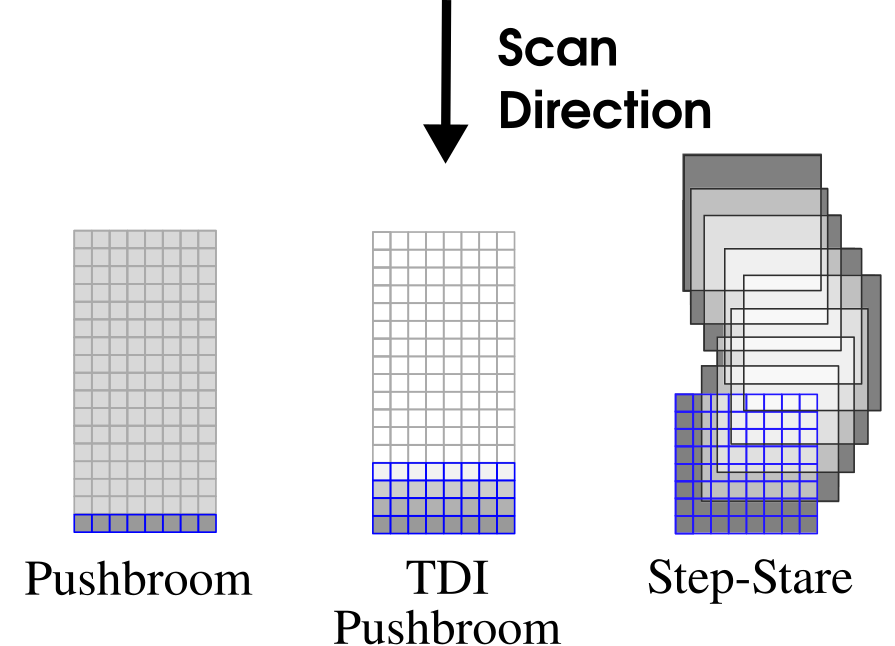
\includegraphics[width=0.42\textwidth]{figures/modalities.png}
\caption{General satellite imaging modalities}
\label{fig:modalities}
\end{figure}

Analog optomechanical stabilization relies on an optomechanical component with the ability to dynamically steer the payload line of sight repetitively so as to remove relative scene motion during integration.  Fast scan mirrors (FSM) or excited dynamic motion of the entire instrument are two ways to achieve this \cite{patent:jonny}, \cite{patent:dirk}.

The analog techniques are considered such because they occur before digital sampling of the detectors and are thus still limited by detector well capacity.  Digital oversampling is not as constrained by $FWC$ because each exposure resets the pixel and thus the $FWC$ can be effectively expanded by as many redundant samples as can be obtained.

Both TDI pushbroom and step-and-stare allow for some form of stabilization or motion compensation which is required to obtain reasonable $SNR$ in high resolution systems.  In the case of Figure~\ref{fig:modalities}, analog charge transfer is depicted for TDI pushbroom, and digital oversampling (through overlapping frames) is depicted for step-and-stare.  Pushbroom is shown mostly for historical reference as pure pushbroom collection is not feasible in systems with $GSD$ much below 10 m.

To date, analog electronic or TDI stabilization has only been implemented successfully in CCD detectors.  There is ongoing work to implement TDI in CMOS detectors but this technology is still immature -- see~\cite{jerram},\cite{rushton}.

Likewise digital oversampling is typically not practical using CCD sensors in high resolution systems due to the inherent limitations on read-out rate of CCD as compared with CMOS technology.

Finally it is important to point out that digital and analog stabilization can be combined in the same system.  Such hybrid stabilization schemes could be in the form of analog opto-mechanical stabilization plus digital oversampling or a TDI CCD that is read out fast enough to allow digital oversampling.  Indeed we will argue later that such hybrid stabilization schemes uniquely leverage the capabilities of modern CMOS detectors, enable smaller systems and provide significant system-level flexibility.

\subsection{Analog Stabilization with TDI}

TDI systems are based on a unique property of CCD image sensors - their ability to move charge between nodes at very high charge transfer efficiency (CTI) and without incurring significant noise in the process.  In fact TDI sensors essentially enabled the move away from film in the classified systems of the 1970's.

Typical TDI sensors will have anywhere from 4 to 256 ``stages,'' each consisting of a row of pixels covering the swath width.  The rows are oriented normal to the scan direction and charge is shifted row-to-row synchronously with the scene motion such that the effective integration time for a point on the ground is multiplied by the number of stages in the device.  Figure~\ref{fig:tdi} illustrates this mode for a 12-stage TDI detector in t-x space where x is in-track dimension.

\includefigure{figures/tdi.pgf}{fig:tdi}{TDI t-x diagram.  Red row indicates one in-track ground sample.}

In general TDI system's photon collection efficacy is ``well-depth limited'' meaning that the duration of integration is typically limited by pixel well saturation before other factors such as number of TDI stages, dark current, or charge transfer efficiency.  For an appropriately exposed scene, the well-limited signal level is:
\begin{equation}
s = \alpha N_{e^-}^{FWC}
\label{eq:well_limited}.
\end{equation}

Noting that the exposure time for a single stage of a TDI system is extrinsically related to the linerate $LR$,
\begin{equation}
t_{int}^{line} = \frac{1}{LR}
\label{eq:lr_tint}.
\end{equation}

and noting that $t_{int} = N_{TDI}t_{int}^{line}$, we can combine with equation \eqref{eq:s} to obtain an expression for optimal number of TDI stages:
\begin{equation}
N_{TDI} =\frac{N_{e^-}^{FWC} Q^2}{k_{pe} L_{sat}}\frac{LR}{QE} \propto \frac{N_{e^-}^{FWC}V_{gnd}}{GSD}
\label{eq:n_tdi}.
\end{equation}
%Figure~\ref{fig:n_tdi} below shows this trade.

%\includefigure{figures/LR_req.pgf}{fig:n_tdi}{TDI linerate required vs. resolution for different pixel well depths}

While extremely powerful and well-proven over many missions, TDI detectors present challenges for low-cost, high resolution missions.

Historically missions have developed custom TDI detectors due to the unique performance and mission requirements of a spacecraft~\cite{jerram}.  These include high line rates, large full-well capacity, low read-noise, high quantum-efficiency and radiation tolerance.  The challenge with CCD-based detectors is data read-out rate which is often limiting for high resolution systems.

In Section \ref{sec:fp_dimensions} we argue that smaller pixels are desirable from a system-size perspective but this typically comes at the expense of pixel full-well capacity, especially in off-the-shelf detectors.  
While  this limitation can be overcome through digital oversampling (Section~\ref{sec:eta_ph}), single TDI detectors inherently couple read-out with integration, precluding this. 

Finally, line-of-sight stability is crucially important during integration in a TDI array \cite{pittelkau} and the charge-transfer process itself incurs smear\cite{fiete_blur}, degrading image MTF.  Digital oversampling partially mitigates both of these issues.

\subsection{Digital Stabilization with Step-and-Stare}
Step and stare relies on a high speed framing CMOS sensor to capture multiple, overlapping frames of the same point on the ground as the scene moves by.  The redundant samples are then re-combined in post-processing to creat output data with a longer effective integration time -- virtual TDI in a way.

\includefigure{figures/step_stare.pgf}{fig:step_stare}{Step-and-stare t-x diagram.  Red row indicates one in-track ground sample}

Figure~\ref{fig:step_stare} illustrates this mode on a t-x diagram.  Note that for visualization we illustrate a detector height of only 36 pixels and a very high framing rate whereas in reality most modern framing sensors are $>$ 1000 pixels high and frames at about 1/6 of the rate shown.  Figure~\ref{fig:step_stare_real} shows the same thing with realistic frame height and framerate.

It is worth noting in this diagram that the photon collection duty cycle, $\phi_{int}$ is small, especially compared with a traditional TDI system which is essentially 100\%.  This can be seen in the white gaps between integration windows.  It is also worth noting the slanted integration periods indicative of motion blur during integration.  Single frame integration time (and thus SNR) for step-and-stare is typically blur-limited (see~\ref{sec:eta_ph}).  This is a problematic limitation and severe enough that systems $GSD$ below about 3~m must reduce $V_{gnd}$ with a bus ``back-nod'' in order to get sufficient signal without incurring substantial blur.

\includefigure{figures/step_stare_real.pgf}{fig:step_stare_real}{Step-and-stare t-x diagram with realistic array height and framerate.}

However digital oversampling through step-and-stare IS NOT limited by small pixel FWC, as the well is read out in each independent integration and then summed digitally.  This means that, in principle, much higher dynamic range can be achieved with small pixels and at high SNR.  To realize this requires analog stabilization to move into the FWC-constrained regime as will be discussed in Section~\ref{sec:eta_ph}.

\subsection{Hybrid Stabilization}

The final modality we will discuss is a hybrid of analog and digital oversampling.  This combination eliminates the shortcomings each have alone and provides a great range of flexibility in both the design and operational space of imaging system.

More specifically, the issues hybrid stabilization addresses are:

\begin{itemize}
    \item Analog stabilization allows operation in FWC-constrained regime, thus extracting the most from optics ($A\Omega$) and detectors ($\eta_{ph}$)
    \item Digital oversampling enables HDR and ``flatter'' $SNR$ over dynamic range as discussed in Section~\ref{sec:hdr}
    \item Digital oversampling allows for resolution-enhancement techniques such as superresolution
    \item Hybrid imaging systems inherently un-constrain other elements of the system in both development and operation allowing for image quality, area collection rate, data intensity, required ACS stability and more to be traded throughout the lifecycle of the system
\end{itemize}

\includefigure{figures/stab_step_stare.pgf}{fig:stab_step_stare}{Stabilized Step-and-Stare t-x diagram.  Red row indicates one in-track ground sample}

Figure~\ref{fig:stab_step_stare} illustrates such hybrid collection in t-x space.  Note the tall collection columns characteristic of a step-and-stare system and the much larger photon collection duty cycle, $\phi_{int}$ characteristic of analog stabilization.  

There are multiple system configurations that allow hybrid stabilization.  The detector must be a staring format with enough rows and high enough framerate to allow for digital oversampling.  While not out of the question in medium and low resolution systems, CCD's typically do not have the read-out rate to accomplish this in high resolution systems.  For staring sensors the linerate, $LR$ in equation \eqref{eq:N_s} is given by

\begin{equation}
\label{eq:lr_framing}    
LR = \left(v_{pix}FPS\right)_{det}.
\end{equation}

Analog stabilization in a staring sensor system can be accomplished in one of three ways

\begin{enumerate}
    \item Optomechanical line-of-sight steering element within the optical chain (e.g. fast scanning mirror, detector translation mechanism) \cite{patent:dirk}
    \item Entire payload or instrument-level actuation to achieve back-scan during integration \cite{patent:jonny}
    \item Inter-row charge transfer in a staring sensor that supports it (TDI-mode)
\end{enumerate}

The third option is attractive from a simplicity perspective but the authors are unaware of staring sensors that both support such a charge transfer mode and have sufficient digital read-out rates to enable digital oversampling in high resolution systems.

Alternatively, multiple TDI push-broom arrays with separate digital read-outs mosaic'd in-track could accomplish digital oversampling.  The oversampling ratio in this case would simply be the number of independent detectors integrated.

The authors belief is that the most promising path to realization are high framerate CMOS detectors coupled with either option 1 or 2.

\section{Performance Trade Space}
\label{sec:trade_space}

The remote-sensing trade space is largely constrained by four mission needs:

\begin{enumerate}
\item Phenomenology
\item Image Quality
\item Collection Capacity
\item Cost
\end{enumerate}

\emph{Phenomenology} refers to the study of the phenomenon being sensed and goes beyond Image Quality to include things like the spectral content of the sensed data.  We will largely discuss the trade space in terms of wide-bandwidth ($>100 nm$) collection in the near-visible spectrum ($\sim 400 nm$ to $\sim 1000 nm$) but will also point out where the trends in questions impact the ability to perform other phenomenology (e.g. SWIR or HSI).  It is also worth pointing out that staring sensors enable video-mode collection, a phenomenology new to space-based remote sensing.

As discussed in Section \ref{sec:modalities} and \ref{sec:entendue} \emph{Image Quality (IQ)} and \emph{Collection Capacity} are tightly coupled at the system level.  Equation ~\eqref{eq:acr_snr_gsd} demonstrates this deep relationship for a set of other system parameters.  In this section we develop this result as it pertains to more granular system parameters.  

\subsection{Q and Pixel Size}

We will study the effect of pixel size through the lens of $Q$ recognizing that \cite{fiete}
\begin{equation*}
    Q = \frac{\lambda f}{D_{ap} p_{px}}.
\end{equation*}

%and then show why driving Q with pixel size is preferable to focal length, $f$ or diameter, D.

$Q$ is generally chosen as a trade between image quality, collection capacity and system size.  

%In~\ref{sec:iq} we show that the NIIRS as predicted by the Generalized Image Quality Equation (GIQE-5) is a useful image quality metric for remote sensing systems.

\includefigure{figures/Q_iq.pgf}{fig:q_iq}{Parametric study of GIQE-5 shows how optimal image quality depends on Q.  Note that this plot assumes $RER_0 = 0.3$ and $GSD = 1m$ for $Q=1$ and that $SNR \sim 1 / Q$}

One thing demonstrated in parametric study of the GIQE-5 is that image quality is often maximized at $Q>1$ (Figure~\ref{fig:q_iq}).  This has also been validated in human-interpreter studies \cite{fiete_Q_IQ} and is not unexpected considering that in a diffraction-limited system with $Q<2$, there is contrast passed by the optical system that is not sampled by the detector.  At first blush it seems obvious that, given the cost and difficulty of building larger optics, systems would be designed at $Q>1$.  

However, there are two other system impacts of $Q$ that argue against pushing it higher.

The first is that for CCD-based TDI systems, pixels with sufficient full well capacity ($FWC$) to meet dynamic range and $SNR$ requirements have required $p_{px} >> 10um$.

Smaller pixels typically store less charge, both in the photodector and storage node. In fact to first order~\cite{jerram}
\begin{equation}
  \label{eq:pix_fwc_scaling}  
N_{e^-}^{FWC} \propto p^2,
\end{equation}
and while there are process optimizations that can improve this, these typically are second order to simple area scaling.  Figure~\ref{fig:p_fwc} shows that Equation \eqref{eq:pix_fwc_scaling} describes the upper frontier reasonably well although several recent pixel architectures are significant outliers.

\includefigure{figures/p_fwc.pgf}{fig:p_fwc}{Relationship of $N_{e^-}^{FWC}$ to pixel size, $p_{px}$.  Note that while the upper frontier generally follows Eq.~\eqref{eq:pix_fwc_scaling}, there are notable outliers especially in some of the new CMOS architectures}

The second challenge in pushing $Q$ higher is that given other system constraints (e.g. $SNR$ required, focal plane dimension)

\begin{equation}
    ACR \propto \frac{1}{Q^2}.
\end{equation}

Thus designers have tended to accept lower $Q$, and hence larger $GSD$ and poorer image quality in exchange for manageable optical focal lengths, increased area collection capacity and acceptable $SNR$ and $DR$.

\begin{observation}[$Q > 1$]
Image Quality is optimized for $Q>1$ but because $ACR \sim 1/Q^2$ and systems were pixel-size limited, historical systems typically have been developed at $Q<1$.
\end{observation}

Happily, the trend towards capable commercial framing image detectors with smaller pixels and large read-out rates opens up the opportunity of driving to towards higher $Q$'s where image quality is optimized without significantly impacting system size.

\subsection{Modality effect on $\eta_{ph}$}
\label{sec:eta_ph}

One way to conceptualize the effect of modality on $\eta_{ph}$ is as the time-average (or integral over time) of the blue areas in Figures~\ref{fig:tdi}, \ref{fig:step_stare}, \ref{fig:step_stare_real} and~\ref{fig:stab_step_stare}.  Increasing in-track height of the blue bars with taller arrays helps improve this integral and reducing the gaps between them horizontally (in time) improves this.  TDI has a time-duty cycle of 1 (no horizontal gaps) while step-and-stare typically have much taller arrays.

In order to quantify this it can be shown that
\begin{equation*}
    A_{fov} = \left(\frac{D_{ap}F^\#}{2}\right)^2 \Omega = \frac{f^2 \Omega}{4} ,
\end{equation*}
or 
\begin{equation}
\label{eq:A_fov}
A_{fov} = \left(\frac{D_{ap}F^\#}{2}\right)^2 \pi \theta_{fov}^2 = \pi \frac{f^2 \theta_{fov}^2}{4},
\end{equation}
where $\theta_{fov}$ is the half-cone angle of the field of view in the small angle approximation.

From this, we can derive $\eta_{ph}$ for systems in two regimes: blur constrained and full-well capacity constrained.  The domains are separated by the following criteria:
\begin{align*}
    N_{e^-}^{FWC} &>& \frac{k_{pe}L_{sat}(QE) N_{bl} GSD}{Q^2 V_{gnd}} & \rightarrow &  \textbf{Blur-constrained} \\
    N_{e^-}^{FWC} &\leq& \frac{k_{pe}L_{sat}(QE) N_{bl} GSD}{Q^2 V_{gnd}} & \rightarrow &  \textbf{FWC-constrained}
\end{align*}
Figure~\ref{fig:eta_regime} is a regime map for a set of reasonable parameters.

\includefigure{figures/blur_fwc_regime.pgf}{fig:eta_regime}{Representative regime map as a function of $GSD$ and $V_{gnd}$}

For the full-well capacity-dominated regime
\begin{equation}
    \label{eq:eta_ph_fwc}
    \eta_{ph}^{FWC} = \frac{4\lambda^2 h_{px} N_{e^-}^{FWC} LR}{\pi L_{sat} D_{ap}^2 \theta_{fov}^2 k_{pe}QE},
\end{equation}
which we can simplify to observe
\begin{equation}
    \label{eq:eta_fwc_scaling}
    \eta_{ph}^{FWC} \propto N_{e^-}^{FWC} LR.
\end{equation}

For high resolution systems without analog stabilization or TDI systems with a fixed number of stages, integration time is typically constrained by the high apparent motion in the focal plane rather than the limited FWC of the pixel (Figure~\ref{fig:eta_regime}).  For digital step-and-stare systems without analog stabilization,
\begin{equation}
    \label{eq:eta_ph_blur}
    \eta_{ph}^{bl} = \frac{4\lambda^2 h_{px}N_{bl}(LR)(GSD)}{\pi D_{ap}^2\theta_{fov}^2 Q^2 V_{gnd}},
\end{equation}
Or 
\begin{equation}
    \label{eq:eta_blur_scaling}
    \eta_{ph}^{bl} \propto  \frac{N_{blur} (LR) (GSD^3)}{V_{gnd}}.
\end{equation}

This scaling law is not good for high resolution systems, requiring high $\frac{LR}{V_{gnd}}$ (and commensurate large data intensity, $I_{D}$, $N_{bl} >> 1 \: \textrm{px}$ or very low $Q$.

Likewise, for a TDI system with a fixed number of stages
\begin{equation}
    \eta_{ph}^{TDI} = \frac{4\lambda^2 h_{px} N_{TDI}}{\pi D_{ap}^2 \theta_{fov}^2 Q^2},
\end{equation}
and we note that 
\begin{equation}
    \label{eq:eta_ph_tdi_scaling}
    \eta_{ph}^{TDI} \propto N_{TDI} GSD^2,
\end{equation}
indicating that $\eta_{ph}$ is highly sensitive to $GSD$ when there is a non-FWC-based integration time constraint.

\begin{observation}[Design for FWC-limited regime]
Operation in the FWC-limited regime results in higher $\eta_{ph}$ and thus should be a design goal.
\end{observation}

In order to operate in the FWC-constrained regime for some resolution, effective scan speed, $V_{gnd}$ must be reduced.  While bus back-nod accomplishes this, it does so at the expense of $ACR$.

\begin{observation}[The need for analog stabilization]
Analog stabilization -- defined as the dynamic cancellation of ground scan speed, $V_{gnd}$ -- is likely required to operate in the FWC-limited regime for high-resolution satellite remote sensing.
\end{observation}

\subsection{Focal Plane Dimensions}
\label{sec:fp_dimensions}
The required physical dimension of the imaging detector is a critical system-driver for a number of reasons.  First, the larger required detector dimension implies either a physically large semiconductor or an array of smaller detectors.  

Very few large monolithic detectors are produced commercially because typically applications requiring them are very specialized.  They are also expensive due to yield issues associated with large semiconductor dies and often have low frame rates due to poor perimeter/area ratios.

Arrays of smaller off-the-shelf detectors at first seem an attractive alternative.  However, such tiled arrays also suffer from several shortcomings.  First, there is overhead in packaging and electrical connection such that it is difficult in practice to get high effective tiling fill fractions.  This may lead to solutions requiring additional optical components such as mirrors to allow for reasonable physical layout of the detectors.  The arrays must also be individually optically aligned to the optics which can be costly and time consuming. However if these problems are solved, tiled arrays are scalable and leverage COTS components.

Whether the solution is monolithic or a tiled array, it is clear that minimizing the physical dimension of the detector array is important in constraining system size and cost.

Expanding Eq.~\eqref{eq:A_fov}, it can be shown that, for a circular aperture, the illuminated focal plane radius is
\begin{equation}
    \label{eq:r_fp}
    r_{fp} = \frac{f\theta_{fov}}{2} = \frac{p_{px}R\theta}{2 (GSD)}.
\end{equation}

For a detector to span the full width of the illuminated area, it thus must span $2 r_{fp}$. 

Eq. \eqref{eq:r_fp} clearly illustrates how important pixel pitch, $p_{px}$ is to minimizing the physical size of detector arrays and provides the second motivatation for the large push towards smaller pixels.

\begin{observation}[Smaller Pixel]
\label{obs:small_pix}
Smaller pixels enable driving system size down and $Q$ up but require hybrid stabilization (digital + analog) to make practical due to inherently lower signal, $S$, obtained during exposure.
\end{observation}

\subsection{Detector Technology}
\label{sec:detector_tech}

Per Eq.~\eqref{eq:eta_ph_fwc}, we note that 
\begin{equation}
    \eta_{ph}^{FWC} \propto h_{px}N_{e^-}^{FWC}LR.
\end{equation}

High efficiency FWC-limited systems must either have larger full-well capacities or higher line-rates.  We observed also that smaller pixels have positive system-level size (and thus cost) impacts and thus one desires focal planes with small pixels and high effective line-rates (where effective line-rates for staring arrays is defined in Eq.~\eqref{eq:lr_framing}).

We also showed in Eq.~\eqref{eq:I_D_scaling} that data pixel FWC is very important to dynamic range and data intensity.

In light of these observations we define a sensor figure of merit
\begin{equation}
    \psi_{px} = h_{px}N_{e^-}^{FWC}LR%\frac{h_{px}N_{e^-}^{FWC}LR}{p_{px}}
    \label{eq:psi_px}.
\end{equation}
$\psi_{px}$ is computed for a number of commercial-off-the-shelf sensors and plotted in Figure~\ref{fig:psi_px}.

\includefigure{figures/p_kpi.pgf}{fig:psi_px}{Detector figure of merit, $\psi_{px}$.  Note log scale and general trend of higher $\psi_{px}$ for CMOS sensors.}

\begin{observation}[CMOS detectors coupled with analog stabilization are enabling]
The trend towards small pixels and high read-out rates enables CMOS detectors to extract more information from high performance, compact (and thus low cost) optics.
\end{observation}

Of course, this additional information does come at the cost of increased data intensity as shown in Equation \eqref{eq:I_D_phi} and, empirically across all types of sensors, in Figure~\ref{fig:psi_vs_id}.

\begin{equation}
\label{eq:I_D_phi}
    I_D \propto \frac{\psi_{px}}{\left(N_{e^-}^{FWC}\right)^3 ACR}
\end{equation}

\begin{figure}
  % Note:  This figure was generated from python script sensors_id.py, included here in sharelatex
  \includegraphics[]{figures/psi_vs_id.pgf}
  \caption{Detector figure of merit is closely correlated with Data Intensity (as expected from Equation \eqref{eq:I_D_phi}), with slight deviations from the trend due to subtle differences in sensor characteristics like aspect ratio and the ratio of well depth to bit depth. CCDs occupy the lower-left corner of the plot, suggesting they are applicable for bandwidth-starved systems that cannot do on-board data fusion.
  \label{fig:psi_vs_id}}
\end{figure}

Systems that are downlink-constrained, therefore, will likely be unable to take advantage of the greater information throughput of newer sensors. Equation \eqref{eq:I_D_phi}  indicates that in these cases, choosing a sensor with lower framerates and marginally larger pixel FWC is a good trade even if the overall $\psi_{px}$ is substantially lower.  Indeed if downlink bandwidth is the largest constraint, Equation \eqref{eq:I_D_phi} suggests that $N_{e^-}^{FWC}$ is probably the most important sensor metric.

One way around this limitation is to shift more of the data reduction onto the spacecraft, for example by performing on-board stacking of digitally-oversampled data. As shown in Figure~\ref{fig:psi_vs_id_summed}, stacking redundant samples prior to downlinking the data reduces the data intensity for a given quantity of information, with detectors that rely more heavily on framerate rather than well capacity realizing a more significant improvement.

\begin{figure}
  % Note:  This figure was generated from python script sensors_id.py, included here in sharelatex
  \includegraphics[]{figures/psi_vs_id_summed.pgf}
  \caption{If digitally-oversampled images can be combined on-board, then the data intensity can be greatly reduced (with systems that rely heavily on digital oversampling benefitting the most from this improvement). Note that, in the above plot, some CMOS systems can provide substantially more useful information for the same amount of downlinked data as the best CCD systems.
  \label{fig:psi_vs_id_summed}}
\end{figure}

The combination of high-frame-rate sensors and robust on-board processing offers the potential to dramatically increase the usable data that can be obtained from bandwidth-limited systems and enable full utilization of high $\psi_{px}$ sensors.

\subsection{Spectral Bands}
\label{sec:spec}

There are a number of system parameters that can be tuned to take advantage of the additional information content available from high-framerate sensors. It can be used to increase area collection capacity (by increasing the ground scan speed of the boresight), improve dynamic range and signal-to-noise (see \ref{sec:hdr}), or add diagnostic capability through additional spectral bands. A standard architecture for collecting multi-spectral data is to use a multi-stripe filter over the sensor, dividing it into a number of regions of approximately equal in-track extent. Each ground point is sampled as it moves through each of the spectral bands. This technique can be used for both TDI and push-framing sensors. For a system where SNR is FWC-constrained, the number of spectral bands that can be collected with a minimum signal-to-noise ratio $SNR_{min}$ at $L_{typ}$ is

\begin{equation}
    \label{eq:nbands}
    N_{bands} = \frac{\text{floor}\left(\frac{N_{rows}\times GSD\times LR}{V_{gnd}}\right)} {\text{ceil}\left(\frac{SNR_{min}^{2}\times\alpha}{FWC}\right)}
\end{equation}

This is a fundamental characteristic of the system that depends on the selection of high-level system parameters (dynamic range, SNR and GSD) as well as details of the orbit and the sensor. Figure \ref{fig:nbands_1m} shows the number of bands available in a 1m GSD system at 500 km. It is evident that only high-framerate sensors are capable of capturing true multispectral imagery at high resolution in this geometry. For a medium-resolution system, however, this constraint does not apply; as seen in Figure \ref{fig:nbands_4m}, a number of CCDs are capable of reading out quickly enough to capture up to 10 spectral bands.

\begin{figure}
  % Note:  This figure was generated from python script sensors_id.py, included here in sharelatex
  \includegraphics[]{figures/nbands_1m.pgf}
  \caption{In this case, we assume a system with an orbital altitude of 500km, a GSD of 1m, and a FWC-constrained SNR. The focal plane is split into spectral bands of equal in-track extent, where the height of each spectral band is set such that the system is able to achieve an SNR of 100 at Ltyp, with alpha (Lsat/Ltyp) = 5 for each ground point. Note that most systems (CCDs and CMOS sensors) require some amount of digital oversampling to achieve the SNR requirement. Most CCDs struggle to sample each point in more than a single channel, while CMOS sensors offer the possibility of truly multispectral coverage. \label{fig:nbands_1m}}
\end{figure}

\begin{figure}
  % Note:  This figure was generated from python script sensors_id.py, included here in sharelatex
  \includegraphics[]{figures/nbands_4m.pgf}
  \caption{Note that, for a GSD of 4m, CCDs are a much more appropriate choice, as there are a number that are capable of multispectral imaging. While the plot suggests that the greater capacity of CMOS sensors may be leveraged by building hyperspectral imagers, in practice this approach requires bandpass filtering that may take the system out of the FWC-limited regime.
  \label{fig:nbands_4m}}
\end{figure}


\subsection{High Dynamic Range Imaging}
\label{sec:hdr}

As mentioned previously, digital oversampling allows improvements in SNR. Previous analysis assumed constant integration times for each of the redundant images, and it was shown that SNR scaled with the square root of the number of redundant samples. Here we demonstrate the advantages of digital oversampling using \emph{different} integration times, and how it leads to high dynamic range imaging by shaping the SNR profile across a range of scene brightness.

In general photography, \emph{exposure bracketing} -- namely, taking multiple pictures of a scene with different exposures -- has been around for a long time, and in the last few decades has evolved to the point today where we see typical consumer camera phones digitally combining images taken with different exposures in near real time.

When digitally oversampling with a constant integration time, every frame is capturing the same range of brightness values.  The maximum brightness (without sensor saturation) is fixed, and SNR is simply being scaled according to the square root of the number of samples.  Note that the SNR for very bright parts of the scene, which are already high due to the nature of photon shot noise, are scaled by the same amount as the dark parts of the scene, which have much lower SNR. Distribution of brightness is scene dependent, but it is often the case that a large fraction of scene content is relatively dark compared to the bright objects in the same scene.  With constant integration time, to capture the dark content with high SNR requires either longer integration times at the cost of clipped scene highlights, or additional oversampling at the cost of data intensity (and perhaps collect capacity due to slower $V_{gnd}$).

Using different integration times resolves the above dilemma: Shorter integration times can capture the brightest areas in the scene, longer integration times can capture the darker areas in the scene, and digital combination of all exposures yields images that combine the best of the short and long integrations, and everything in between.  Figure~\ref{fig:hdr_snr_example} demonstrates the concepts from the point of view of SNR. In the figure are the SNR profiles of three exposures:  A ``nominal'' exposure (1x), an exposure with double the nominal integration time (2x), and an exposure with quadruple the nominal integration time (4x). The 1x exposure captures some range of brightness values, normalized to maximum value of 1.0, with an SNR dependence on brightness that assumes photon shot noise as the dominant noise source. The 2x integration captures only half the range of brightness values, but has 1.4 times the SNR over that range; similarly, the 4x integration only captures one quarter the full range of brightness, but has double the SNR over that range.

\begin{figure}
  % Note:  This figure was generated from Matlab script hdr_jonny_paper.m, included here in sharelatex
  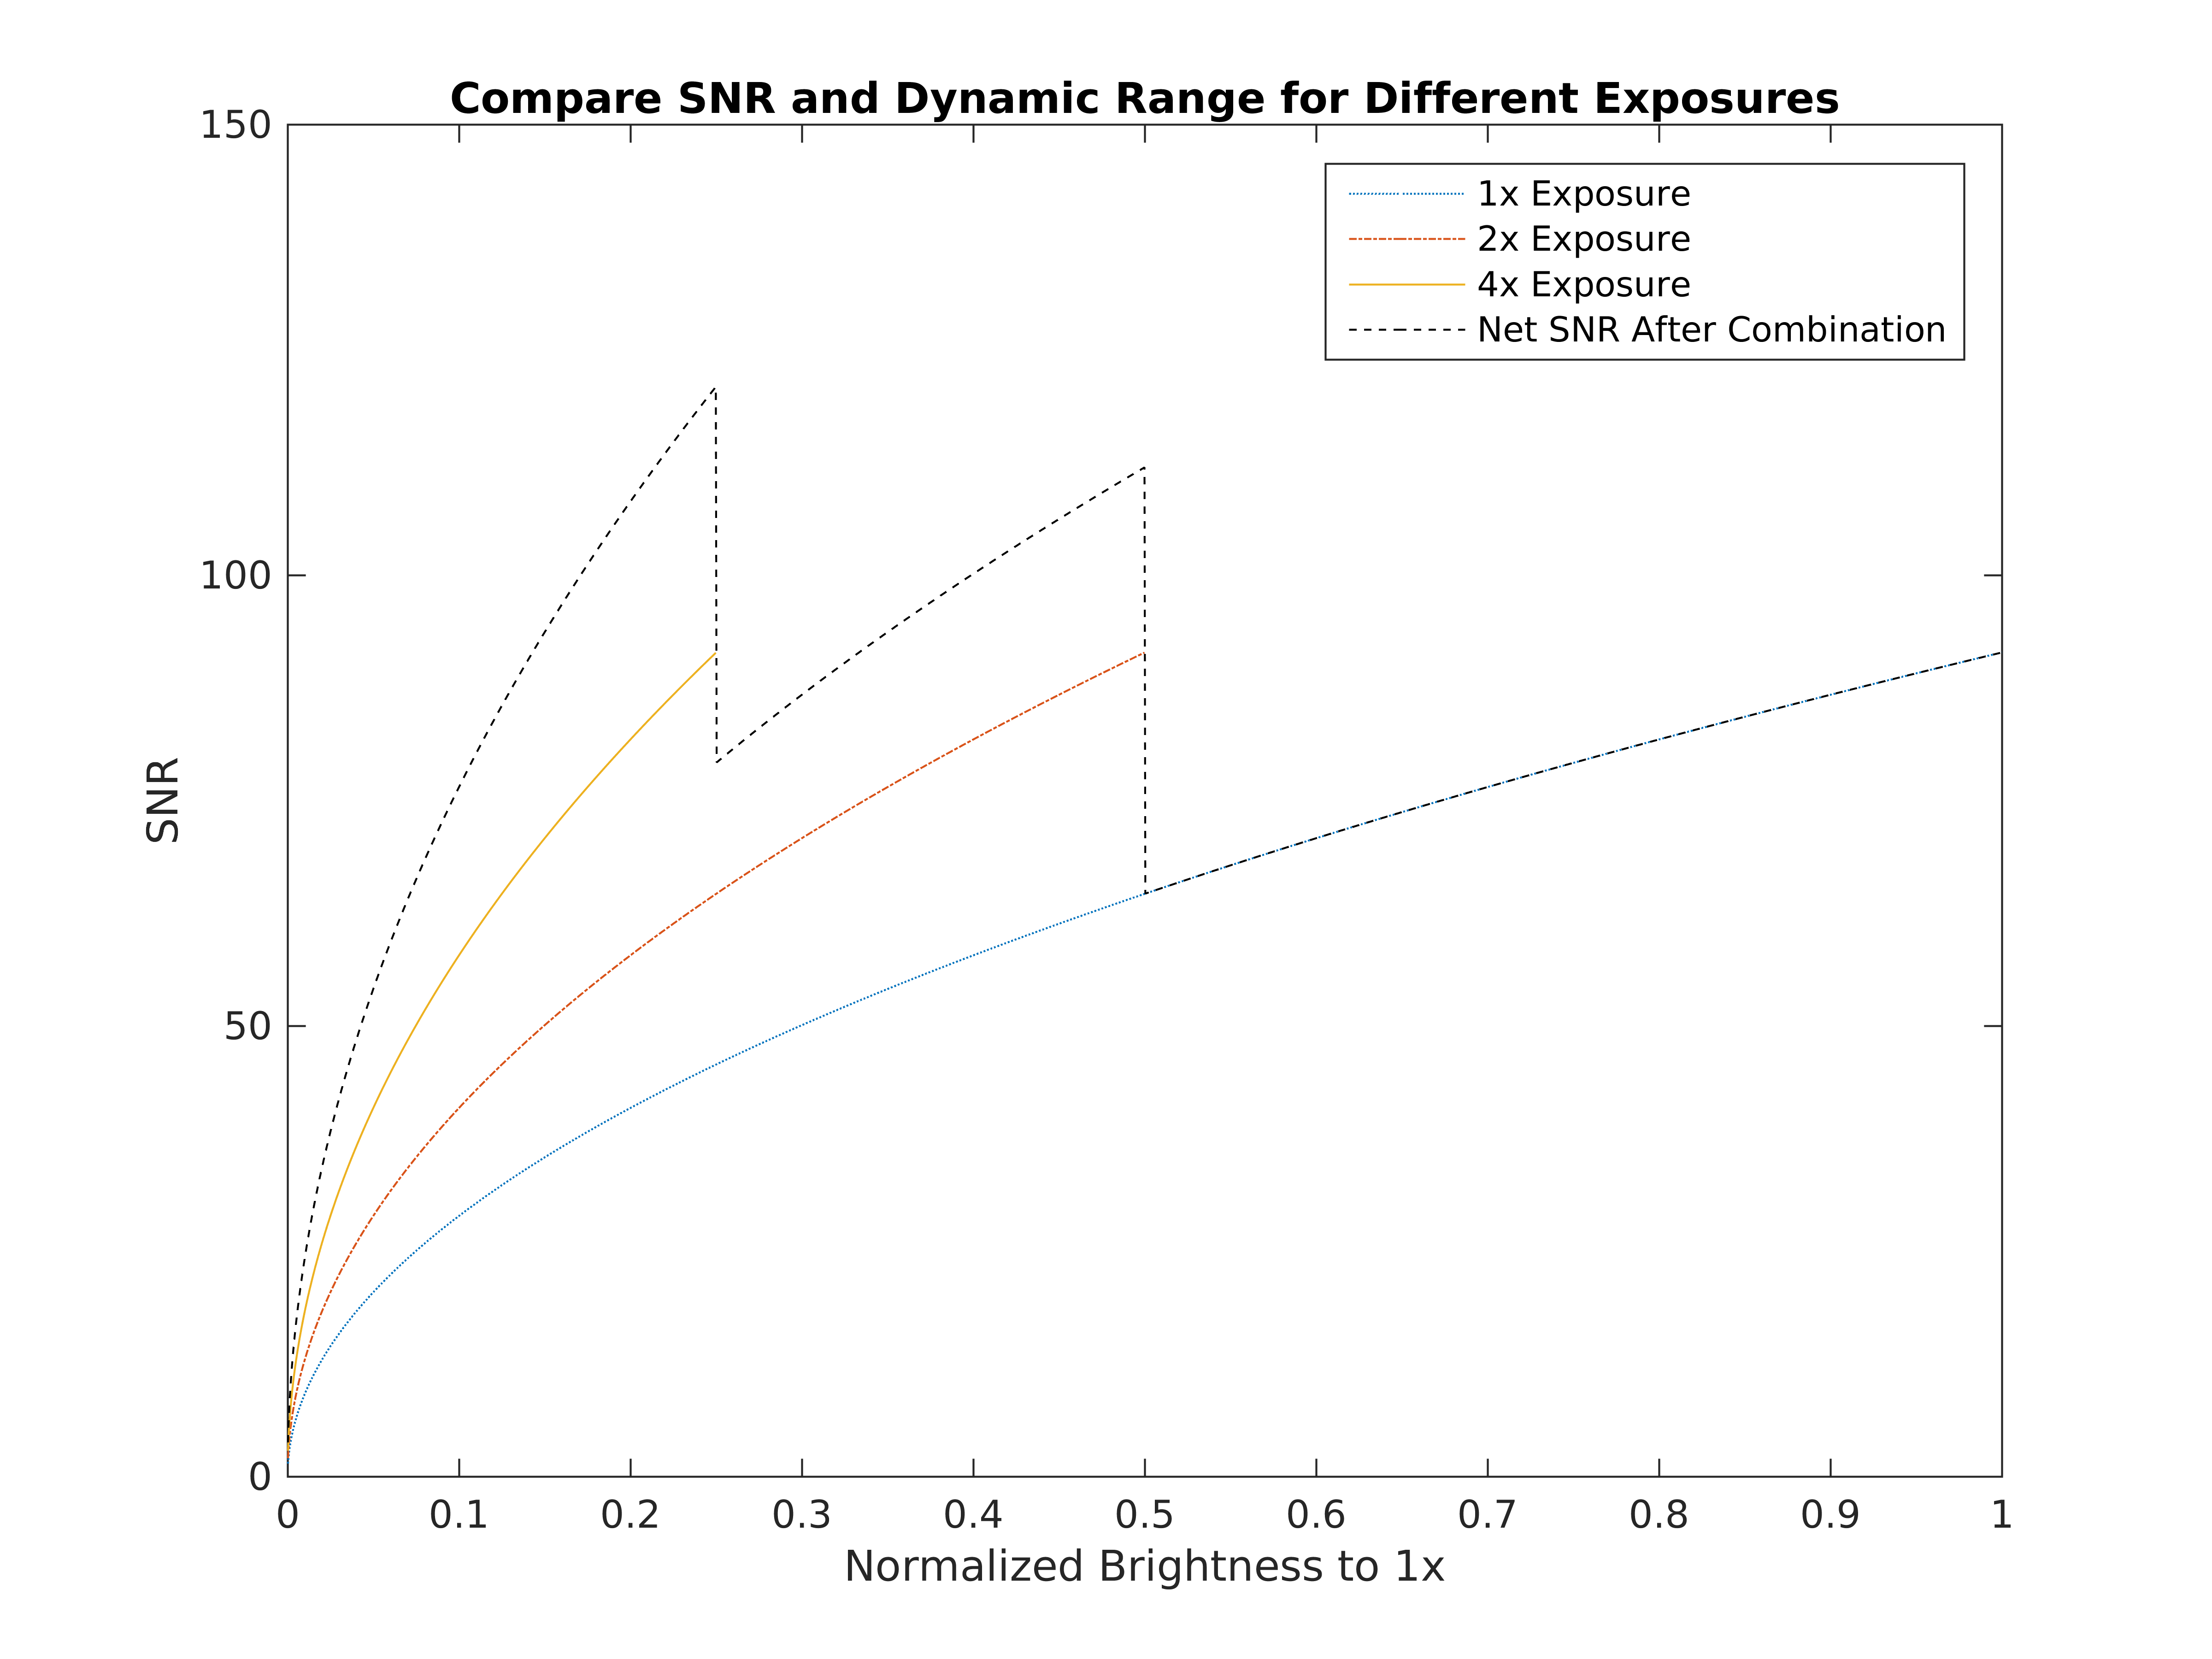
\includegraphics[width=\columnwidth]{figures/hdr-design-snr-hdr-examples.png}
  \caption{SNR and dynamic range for different integration times. The nominal 1x integration time captures a range of bright levels up to 1.0.  Longer integration times capture smaller ranges of brightness, but with higher SNR. Combining the three image exposures gives the saw-tooth-shaped SNR profile. \label{fig:hdr_snr_example}}
\end{figure}

Combining the three exposures from Figure~\ref{fig:hdr_snr_example} yields an effective SNR profile as shown by the saw-tooth dashed line in the figure. This composite SNR assumes a straightforward maximum-likelihood approach to combining images taken with different integration times, and does not include any advanced processing such as super-resolution, deblurring, or noise reduction. Note that in this hypothetical case, some darker regions in a scene have \emph{higher} SNR than some brighter regions of the scene, and is quite distinct from the SNR behavior of simple shot noise.

\begin{figure}
  % Note:  This figure was generated from python script hdrfigs.py, included here in sharelatex
  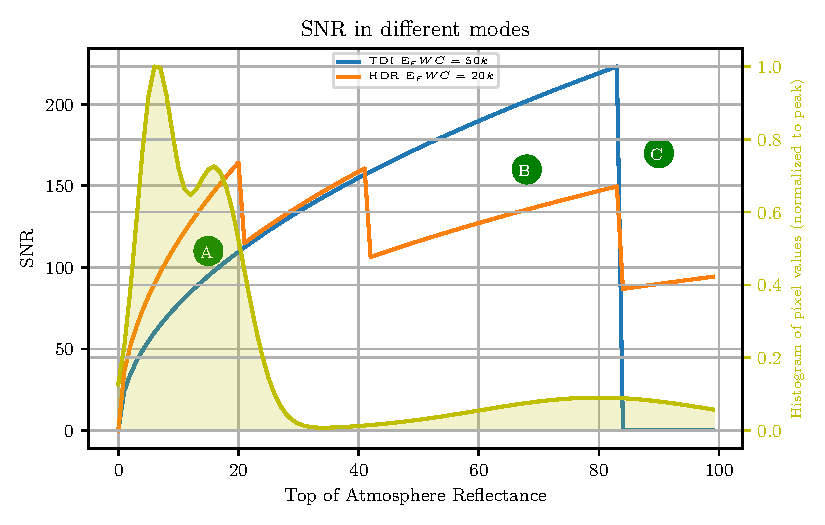
\includegraphics[]{figures/snr_vs_L.pgf}
  \caption{The SNR as a function of scene luminosity for a TDI-based system using a CCD with a FWC of 5e4 electrons, and for a digitally-oversampled system using 4 different HDR integration times on a CMOS sensor with a FWC of 2e4 electrons. Also shown is the luminosity histogram for a typical scene. In region A (relatively low luminosity), the stabilized HDR system is able to achieve a substantially higher SNR than the TDI system thanks to the ability to take long integrations. In region B (relatively high luminosity), the TDI system has higher SNR; however, there is minimal practical advantage, since there is relatively little scene content in this regime, and the extra SNR is above the “good enough” level that the HDR system can capture. In region C (highlights and specular reflections), the TDI system is saturated and reports no useful signal, while the HDR system is still able to discriminate contrast within the highlights. \label{fig:snr_vs_L}}
\end{figure}

More than simply increasing the dynamic range of the output data product, allowing different integration times grants considerable flexibility in tuning image quality. Figure~\ref{fig:snr_vs_L} illustrates the power of this approach. In a typical scene, the majority of the content has a luminosity much lower than the saturation value, and $\alpha$ is between 4-16. For a single-shot image, the signal-to-noise ratio for most of the pixels of interest is therefore 2-4 times lower than the FWC-limited SNR of the sensor. Even a relatively small amount of digital oversampling, using a sensor with a much smaller FWC, allows a system to achieve a higher SNR in the luminance range where most of the content lies. 

\begin{figure}
  % Note:  This figure was generated from python script hdrfigs.py, included here in sharelatex
  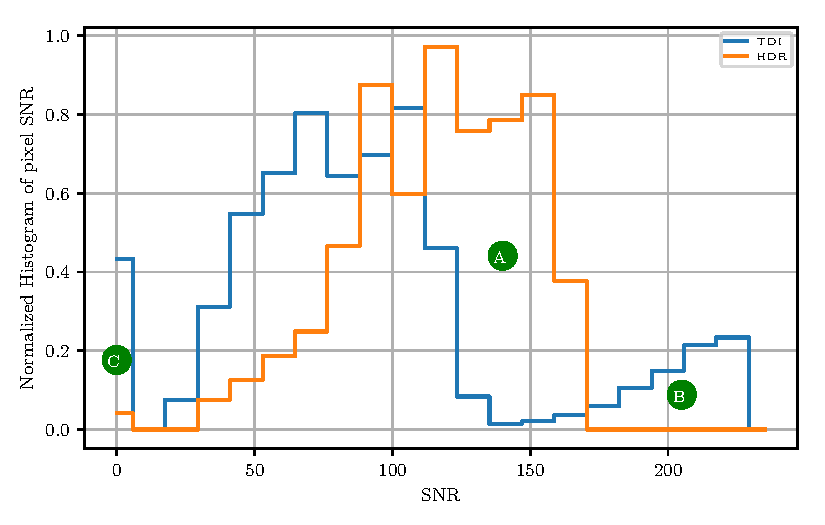
\includegraphics[]{figures/hist_vs_snr.pgf}
  \caption{Histogram of SNR values assuming the scene luminosity histogram and luminosity-to-SNR mapping of the two systems in Figure A. Note the HDR system observes the bulk of the scene in the “sweet spot” of high SNR, while the TDI system has a lower mean SNR along with a substantial “blind spot” for highlights.  \label{fig:hist_vs_snr}}
\end{figure}

Figure~\ref{fig:hist_vs_snr} shows the resulting distribution of SNR for all the pixels in the image. The simple HDR system produces a uniform, high SNR for the bulk of the pixels in the scene, while the single-shot image suffers from saturation of highlights and underexposure (low SNR) for much of the scene. Indeed, this is a best-case scenario for single-shot (or TDI) system, in that we have assumed that the integration time has been tuned perfectly to the desired saturation radiance; if there are errors in the exposure model, the SNR distribution will be shifted to produce either more severe saturation or more underexposure. The HDR scheme can be configured to optimize SNR over an extremely wide range of luminance values.

%Figure~\ref{fig:hdr_snr_flatter} shows the result of choosing integration times to maximize ``flatness'' of the SNR curve when combining 16 images, and compares that to the case of combining 16 images of fixed integration time. The trade-off in this example was to sacrifice SNR in the brightest regions, where less data resides and where the SNR was already relative high, in exchange for higher SNR in the low-lights, where more of the scene content likely resides. There are many other possible criteria one might use to optimize integration times.

%\begin{figure}
%  % Note:  This figure was generated from Matlab script hdr_jonny_paper.m, included here in sharelatex
%  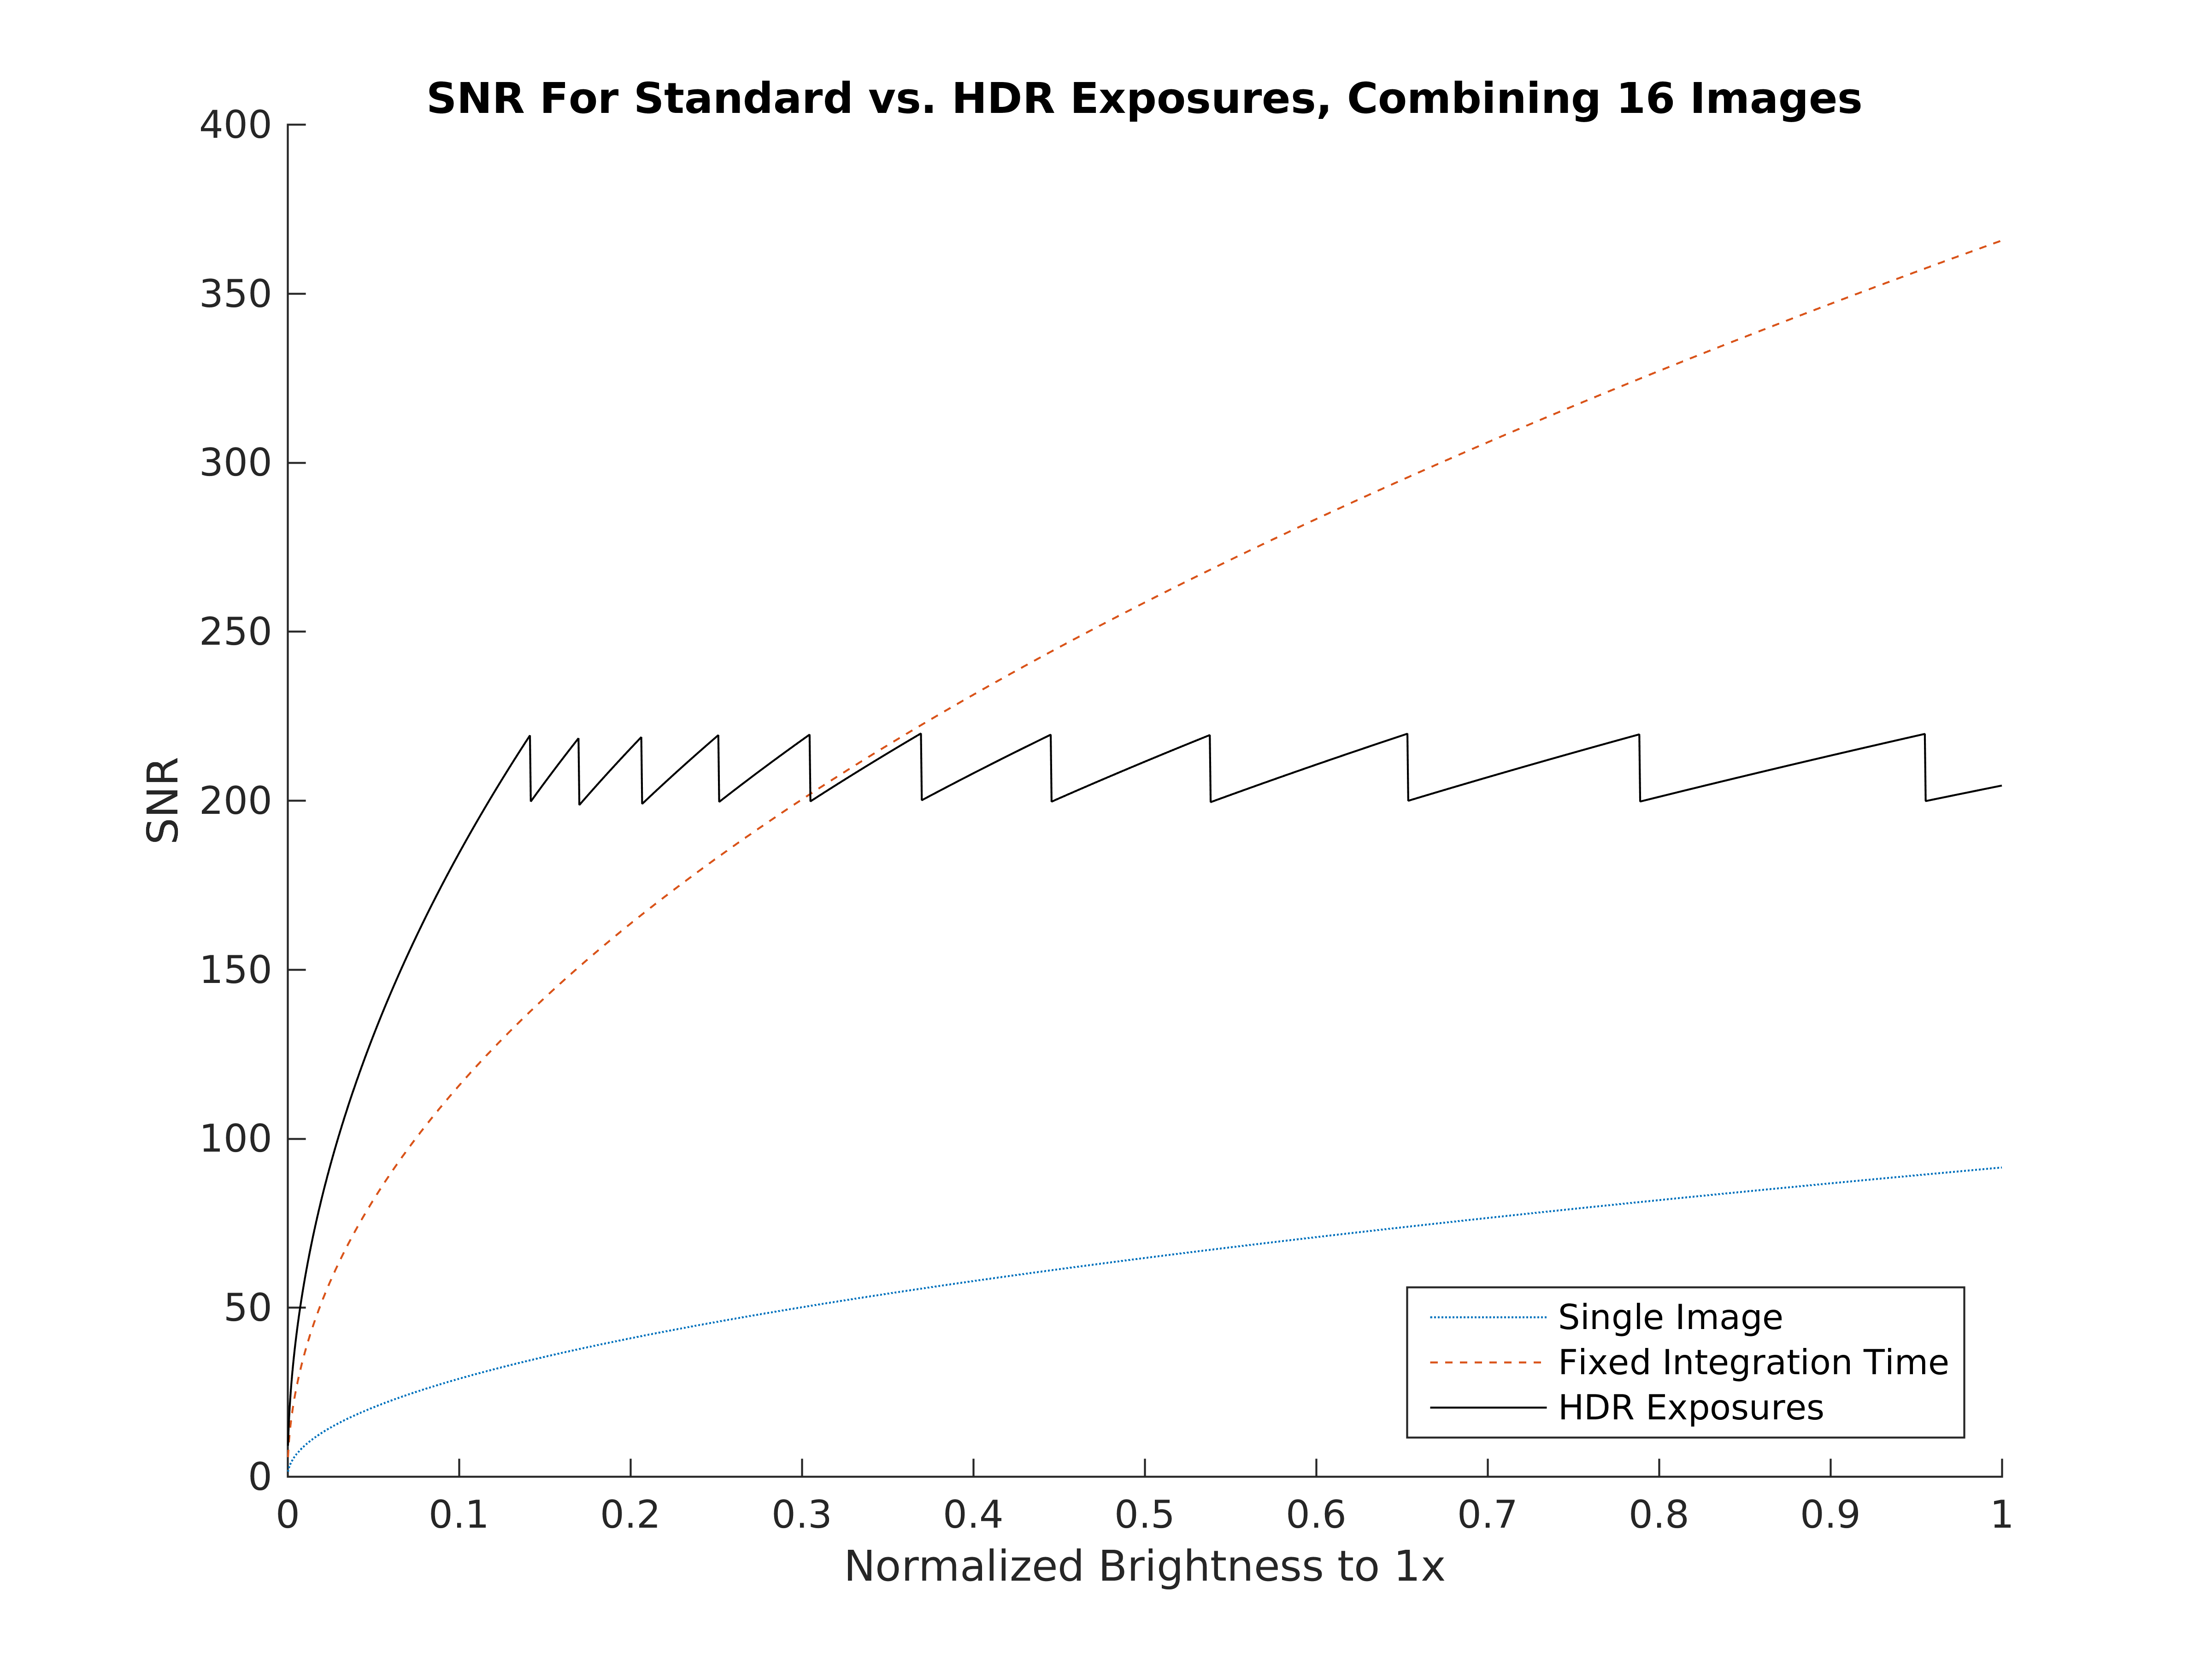
\includegraphics[width=\columnwidth]{figures/hdr-design-compare-snr.png}
%  \caption{Example SNR profiles of combining 16 images, with comparison of combining (1)~fixed integrations times, and (2)~variable integration times.\label{fig:hdr_snr_flatter}}
%\end{figure}


\subsection{Comparison of Modalities}
In summary, we have shown that the hybrid stabilization imaging modality has some strong advantages over pure analog or digital stabilization.  Specifically hybrid stabilization

\begin{enumerate}
\item Leverages the high $\psi_{px}$ of newer sensors 
\item Enables operation in the FWC-limited regime 
\item Expands dynamic range and $SNR$ beyond the native sensor capacity 
\item Provides the designer with additional parameters that can be used to trade image quality, capacity and data intensity through the entire system lifecycle (even in operation)
\end{enumerate}

Table~\ref{table:modalities} summarizes qualitatively the relative advantages and disadvantages of the three modalities.

\begin{table}[ht]
\resizebox{.45\textwidth}{!}{%
\centering
\begin{tabular}{@{}rccccc@{}}
\multicolumn{1}{l}{}                                                 & \textbf{DR}                       & \textbf{SNR}                        & $\eta_{ph}$         & \textbf{\begin{tabular}[c]{@{}c@{}}Stability\\ Req'd\end{tabular}} & \textbf{\begin{tabular}[c]{@{}c@{}}Data\\ Intensity\end{tabular}} \\ \cmidrule(l){2-6} 
\textbf{\begin{tabular}[c]{@{}r@{}}Analog \\Electronic\end{tabular}}                                                         & {\color[HTML]{F56B00} \textbf{-}} & {\color[HTML]{32CB00} \textbf{+}}   & {\color[HTML]{FE0000} \textbf{-}} & {\color[HTML]{FE0000} \textbf{- -}}                                & {\color[HTML]{32CB00} \textbf{++}}                                \\ \midrule
\textbf{\begin{tabular}[c]{@{}r@{}}Digital\\Oversampling\end{tabular}}                                                  & {\color[HTML]{32CB00} \textbf{+}} & {\color[HTML]{32CB00} \textbf{+}} & {\color[HTML]{FE0000} \textbf{-}} & {\color[HTML]{32CB00} \textbf{++}}                                 & {\color[HTML]{FE0000} \textbf{- -}}                               \\ \midrule
\textbf{Hybrid} & {\color[HTML]{32CB00} \textbf{+}} & {\color[HTML]{32CB00} \textbf{++}}  & {\color[HTML]{32CB00} \textbf{+}} & {\color[HTML]{32CB00} \textbf{Tunable}}                            & {\color[HTML]{32CB00} \textbf{Tunable}}                           \\ \bottomrule
\end{tabular}%
}
\caption{Relative advantages and disadvantages of the modalities. $DR$ is dynamic range, $SNR$ is signal-to-noise ratio.}
\label{table:modalities}
\end{table}

\section{Design Case Studies}
\label{sec:case_studies}

In this section we take the earlier results and apply them to two systems: a very high resolution small satellite for point-collection and a high resolution large area collector for mapping.  For both case studies, we use the following assumptions:

\begin{itemize}
    \item Goal is to meet requirements while minimizing overall system size, which is driven directly by aperture diameter and focal plane size
    \item Imaging performance is defined by GIQE-based $GRD_{eff}$ or NIIRS
    \item For simplicity, IQ is specified only for panchromatic but it is assumed the focal plane is split in in-track extent equally amongst 5 multi-spectral bands (including PAN) and all bands have identical $GSD$
    \item Dynamic range computed assuming equal exposures -- the authors note that improved dynamic range is possible for digitally stabilized system with bracketed exposures as discussed in Section~\ref{sec:hdr}
\end{itemize}

Additional requirements and assumptions are captured in Table~\ref{table:case_study_reqs}.

\begin{table}[t]
\centering
\resizebox{\linewidth}{!}{%
\begin{tabular}{@{}ccl@{}}
\toprule
\textbf{Requirement} & \textbf{Value}                                                                       & \textbf{Note}              \\ \midrule
Altitude & 500 km &\\ \midrule
$V_{gnd}$ & 7.06 km / sec &\\ \midrule
$\lambda$ & \begin{tabular}[c]{@{}c@{}}450 nm to\\ 800 nm\end{tabular} \\ \midrule
$\lambda_c$ & 525 nm & \\ \midrule
$L$ & \begin{tabular}[c]{@{}c@{}}200 W/m$^2$-sr (sat.)\\ 10 W/m$^2$-sr (typ.)\end{tabular} & Over $\lambda$, see \cite{morfitt2015landsat} \\ \midrule
$SNR$ & 70 & at $L_{typ}$ for $\alpha = 0.05$               \\ \midrule
$DR$ & 80 dB & \\ \midrule
$\sigma_{uncorr.}$  & $< 10 \, e^{-}$ RMS & \\ \midrule
Optical Obscuration & 0.3 & By diameter \\ \midrule
Optical WFE & 0.15 $\lambda$ RMS & At $\lambda_c$ \\ \midrule
$N_{\lambda}$ & 5 & PAN+NRGB \\ \midrule
$N_{ct}$ & 5 & $\sim 20$ kpix cross-track req.\\ \bottomrule
\end{tabular}%
}
\caption{Case study requirements and assumptions.}
\label{table:case_study_reqs}
\end{table}

Using the $SNR$ requirement at $L_{typ}$ and saturation at $L_{sat}$ from Table~\ref{table:case_study_reqs} as well as Equation \eqref{eq:snr_alpha_multiframe_simp} we can immediately determine that for any system meeting these requirements,
\begin{equation}
    \left[N_sN_{e^-}^{FWC}\right]_{req} \geq \frac{SNR_{req}^2}{\alpha} = 9.8\times 10^4 \, e^-
    \label{eq:NsNeFWC_req}
\end{equation}

One design choice would be to use an analog-stabilized detector that does not allow digital oversampling (TDI push-broom or staring sensor with $LR < 2\frac{V_{gnd}}{GSD}$) and require $\mathbf{N_{e^-}^{FWC} \geq 9.8\times 10^4 \, e^-}$.  

Unfortunately, at the small pixel sizes there are no known available commercial sensors with sufficient well depth. Therefore a small-system based on COTS detectors is pushed to \textbf{digital oversampling}.  

Additionally, in order to avoid operating in the blur-limited regime we will state without defense (see Figure~\ref{fig:eta_regime}) that all of these systems must have some form of analog stabilization (either TDI or opto-mechanical)

We can connect Equation~\eqref{eq:NsNeFWC_req} and our detector metric, $\psi_{px}$ in Equation~\eqref{eq:psi_px} to show that:
\begin{equation}
    \psi_{px} \geq \frac{h_{px} N_{\lambda} V_{gnd} \left[N_sN_{e^-}^{FWC}\right]_{req}}{GSD \times N_{det}}
    \label{eq:psi_px_req},
\end{equation}
where we introduce $N_{\lambda}$ to denote the number of unique spectral bands the focal plane is divided into in the in-track dimension and $N_{det}$ to denote the number of unique detectors tiled in the focal plane.

\subsection{50-cm Resolution Point Collection Small-Sat}

This design point is for a minimum-size (low-cost) 50cm $GRD_{eff}$ spacecraft with a relatively small cross-track swath width.  High level requirements are captured in Table~\ref{table:50cm_specs}.

\begin{table}[ht]
\centering
\resizebox{\linewidth}{!}{%
\begin{tabular}{@{}lll@{}}
\toprule
\textbf{Requirement} & \textbf{Value} & \textbf{Note}  \\ \midrule
$GRD_{eff}$ & 0.5 m  & at Nadir\\ \midrule
NIIRS & 5.4 & From Eq. \eqref{eq:grd_eff} \\ \midrule
$x_{ct}$ & 7.5 km & \\ \midrule
$Q$ & 1.3 & Compromise between IQ, $\psi_{px}$, $I_D$ \\ \midrule
$N_sN_{e^-}^{FWC}$   & 98 k$e^{-}$ & From $SNR_{\alpha}$, $\alpha$  \\ \bottomrule
\end{tabular}%
}
\caption{Specification for 50-cm small-sat point collector.}
\label{table:50cm_specs}
\end{table}

Note that the first thing we will look at is the required $\psi_{px}$ for the focal plane.  Given the $GRD_{eff}$ (or equivalently, $NIIRS$), $Q$, obscuration and WFE requirements, we use GIQE5 to determine $D_{ap} = 0.48 \, m$, $GSD = 42.5 \, cm$ and $h_{px} \geq 17,698$.

Using Equation \eqref{eq:psi_px_req} we can determine $\psi_{px} \geq \mathbf{1.4 \times 10^{14} \, e^- / s}$ - a requirement higher than any single detector in our survey is capable of (Figure~\ref{fig:psi_px}).  The large number of cross-track pixels required is also a challenge given typical COTS sensor formats.  Happily, we can split the FOV up among a tiled array of detectors to reduce the required $\psi_{px}$ and $h_{px}$ for any one detector.  

The 4K TV standard means that assuming a single detector width of 4,000 pixels is a reasonable first assumption for tiling.  To meet the $h_{px}$ requirement, this would require \textbf{four tiled detectors}.  And now the unit-detector $\psi_{px}$ is reduced by a factor of four to $\mathbf{3.6 \times 10^{13} \, e^-/s}$.  The only sensor in our survey that meets this requirement is the BAE LTN4625a with a $\psi_{px} = \mathbf{5.73 \times 10^{13} \, e^- / s}$.

As we noted before, analog stabilization is required to operate in the FWC-constrained regime making the overall system a hybrid stabilized system.

The full point design given this sensor choice produces the parameters captured in Table~\ref{table:50cm_parameters}.

\begin{table}[h!]
\centering
\resizebox{\linewidth}{!}{%
\begin{tabular}{@{}lll@{}}
\toprule
\textbf{Parameter} & \textbf{Value} & \textbf{Note}  \\ \midrule
$GSD$ & 42 cm & From GIQE optimization \\ \midrule
$D_{ap}$ & 48 cm & From GIQE optimization\\ \midrule
$h_{px}$ & \begin{tabular}[c]{@{}l@{}}18432 (total)\\ 4608 (per sensor)\end{tabular} & From $N_{ct}$, $GSD$ \\ \midrule
$x_{ct}$ & 7.8 km & \\ \midrule
$\psi_{px}^{det}$ & $\geq 3.6\times 10^{13} \, e^-/s$ & \\ \midrule
Focal Plane Width & 96.9mm & \\ \midrule
$FPS^{req}$ & $\geq 96$ & \\ \midrule
$Ns$ & 3 & \\ \midrule
$I_D^{raw}$ & 41.3 bit / pix & Uncompressed \\ \midrule
$DR$ & 82.8 dB & \\\bottomrule
\end{tabular}%
}
\caption{Dependent system parameters for optimized 50cm system}
\label{table:50cm_parameters}
\end{table}

We re-iterate the following observations about this point design:

\begin{enumerate}
    \item The minimum requirements for this system can only be met with small-pixel COTS sensors using hybrid stabilization and high-speed CMOS framing sensors
    \item This system achieves a very high level of image quality (NIIRS 5.4, 42-cm $GSD$, high $SNR$) simultaneously with a high dynamic range of $>$ 82 dB
    \item The cost of this image quality perfmance is a relatively small swath width of 7.8 km and high data intensity of $>$ 41 bit / pix uncompressed.
\end{enumerate}

\subsection{1-m Resolution Large-Area Collector}

For this case study, the design point goal is a 1-m class $GRD_{eff}$ with a large swath width for large area coverage.  Image quality is still considered important and so none of the other requirements ($SNR$, $N_\lambda$, etc) are different than for the 50-cm system.  The requirements for this system are captured in Table~\ref{table:1m_case}. 

\begin{table}[h!]
\centering
\resizebox{\linewidth}{!}{%
\begin{tabular}{@{}lll@{}}
\toprule
\textbf{Requirement} & \textbf{Value} & \textbf{Note}  \\ \midrule
$GRD_{eff}$ & 1.0 m  & at Nadir\\ \midrule
NIIRS & 4.4 & From Eq. \eqref{eq:grd_eff} \\ \midrule
$x_{ct}$ & $\geq$ 20 km & \\ \midrule
$Q$ & 1.3 & Compromise between IQ, $\psi_{px}$, $I_D$ \\ \midrule
$N_sN_{e^-}^{FWC}$   & 98 $ke^{-}$ & From $SNR_{\alpha}$, $\alpha$  \\ \bottomrule
\end{tabular}%
}
\caption{Specification for 1-m large-area collector.}
\label{table:1m_case}
\end{table}

Following the analysis done for the 50cm case, we determine that the required $\psi_{px}$ for this system is $\psi_{px} \geq \mathbf{9.9 \times 10^{13} \, e^-/s}$.  Again this value exceeds any of the surveyed sensors so a tiled array is required.  

We again assume a 4K-wide format sensor as a starting point and note that the cross-track pixel count requirement is $h_{px} \geq 23,966$ and to meet this requires at least six 4,000 pixel wide sensors.

With six sensors, the unit-sensor $\psi_{px}$ requirement is now reduced to $\psi_{px} \geq \mathbf{1.7 \times 10^{13} \, e^-/s}$. This performance is met by five of the surveyed sensors all of which are CMOS.  The GPixel 3005 sensor has an electronic rolling shutter and is thus likely problematic.

Given the choice of sensors, we look at how other system parameters are affected by which sensor is selected in Table~\ref{table:1m_sensor_choice}.

\begin{table}[h!]
\centering
\resizebox{\linewidth}{!}{%
\begin{tabular}{@{}lcccccl@{}}
\toprule
\textbf{Sensor} & \textbf{$N_{det}$} & \textbf{$FPS^{req}$} & \textbf{$x_{ct}$} & \textbf{$DR$} & \textbf{$I_D$} & \textbf{$F^\#$} \\ \midrule
LTN 4625a & 6 & 49 & 23 km & 82.8 dB & 41.3 bit / pix & 13.6 \\
Python 25k & 5 & 75 & 21.2 km & 68.2 dB & 102.0 bit / pix & 11.1 \\
CMV12000 & 6 & 111 & 20.3 km & 69.4 dB & 92.2 bit / pix & 13.6 \\
CMV50000 & 4 & {\color[HTML]{CB0000} \textbf{49.5}} & 26.3 km & 72.8 dB & 84.6 bit / pix & 11.4 \\ \bottomrule
\end{tabular} %
}
\caption{Impact of sensor choice on other system parameters}
\label{table:1m_sensor_choice}
\end{table}

With the exception of the LTN4265a, the biggest downside of most of the sensors is the large data intensity, $I_D$, and relatively low DR -- both driven by the small FWC.

It is also worth pointing out that although the CMV50000 nominally meets the $\psi_{px}$ requirement when we assumed a six detector mosaic, to meet the cross track FOV requirement only requires four such detectors.  And with only four detectors it does not meet the $\psi_{px}$ requirement any longer due to its relatively low frame readout rate of 30 FPS.

Again, we chose the LTN4625a sensor and the resulting system parameters are compiled in Table~\ref{table:1m_parameters}.

\begin{table}[h!]
\centering
\resizebox{\linewidth}{!}{%
\begin{tabular}{@{}lll@{}}
\toprule
\textbf{Parameter} & \textbf{Value} & \textbf{Note}  \\ \midrule
$GSD$ & 83 cm & From GIQE optimization \\ \midrule
$D_{ap}$ & 25 cm & From GIQE optimization\\ \midrule
$h_{px}$ & \begin{tabular}[c]{@{}l@{}}27648 (total)\\ 4608 (per sensor)\end{tabular} & From $N_{ct}$, $GSD$ \\ \midrule
$x_{ct}$ & 23 km & \\ \midrule
$\psi_{px}^{det}$ & $\geq 1.7\times 10^{13} \, e^-/s$ & \\ \midrule
Focal Plane Width & 127.2 mm & \\ \midrule
$FPS^{req}$ & $\geq 49$ & \\ \midrule
$Ns$ & 3 & \\ \midrule
$I_D^{raw}$ & 41.3 bit / pix & Uncompressed \\ \midrule
$DR$ & 82.8 dB & \\\bottomrule
\end{tabular}%
}
\caption{Dependent system parameters for optimized 1-m system}
\label{table:1m_parameters}
\end{table}

\subsection{30-cm Point Collector} 

For fun we will try one more case with the very agressive design goal of a 30-cm $GRD_{eff}$ system.  Iteration shows that some requirements must be relaxed to achieve this case with the sensors available to us and so we will relax the following requirements:
\begin{itemize}
\item Required $SNR$ at $\alpha = 0.05$ reduced from 70 to 50
\item Required dynamic range reduced from 80dB to 75dB
\end{itemize}

The other case-specific direct and derived requirements are captured in Table~\ref{table:30cm_case}. 

\begin{table}[h!]
\centering
\resizebox{\linewidth}{!}{%
\begin{tabular}{@{}lll@{}}
\toprule
\textbf{Requirement} & \textbf{Value} & \textbf{Note}  \\ \midrule
$GRD_{eff}$ & 30 cm  & at Nadir\\ \midrule
NIIRS & 6.1 & From Eq. \eqref{eq:grd_eff} \\ \midrule
$x_{ct}$ & $\geq$ 5 km & \\ \midrule
$Q$ & 1.3 & Compromise between IQ, $\psi_{px}$, $I_D$ \\ \midrule
$N_sN_{e^-}^{FWC}$   & 50 $ke^{-}$ & From $SNR_{\alpha}$, $\alpha$  \\ \bottomrule
\end{tabular}%
}
\caption{Specification for 30 cm point collector}
\label{table:30cm_case}
\end{table}

The model produces a feasible solution to this system design utilizing 5 tiled LTN4625a detectors with the parameters given in Table~\ref{table:30cm_parameters}

\begin{table}[h!]
\centering
\resizebox{\linewidth}{!}{%
\begin{tabular}{@{}lll@{}}
\toprule
\textbf{Parameter} & \textbf{Value} & \textbf{Note}  \\ \midrule
$GSD$ & 23 cm & From GIQE optimization \\ \midrule
$D_{ap}$ & 89 cm & From GIQE optimization\\ \midrule
$h_{px}$ & \begin{tabular}[c]{@{}l@{}}23040 (total)\\ 4608 (per sensor)\end{tabular} & From $N_{ct}$, $GSD$ \\ \midrule
$x_{ct}$ & 5.3 km & \\ \midrule
$\psi_{px}^{det}$ & $\geq 3.4\times 10^{13} \, e^-/s$ & \\ \midrule
Focal Plane Width & 127.2 mm & \\ \midrule
$FPS^{req}$ & $\geq 119$ & \\ \midrule
$Ns$ & 1 & \\ \midrule
$I_D^{raw}$ & 13 bit / pix & Uncompressed \\ \midrule
$DR$ & 78.1 dB & \\\bottomrule
\end{tabular}%
}
\caption{Dependent system parameters for optimized 30 cm system}
\label{table:30cm_parameters}
\end{table}

This is an impressive result considering that this is a system with better $GSD$ than commercial state-of-the-art (WorldView-3, WorldView-4) and that is likely significantly smaller and lower cost than those systems.

\section{Conclusions}
\label{sec:conclusions}

In summary, we have shown that

\begin{enumerate}
    \item The trend in space-based remote sensing is to smaller sized system due to cost and scalability
    \item Small pixel, high data rate commercial CMOS detectors enable high performance systems at reduced size \& cost
    \item To realize potential of modern area detectors, a combination of analog and digital stabilization (hybrid stabilization) is required
    \item Hybrid stabilization with high speed CMOS sensors enables High Dynamic Range imaging in high resolution systems
    \item Hybrid stabilization with high-speed CMOS sensors enable higher spectral dimensionality systems (multi- or hyper- spectral)
\end{enumerate}

The potential of the trends identified here have yet to be fully realized and the authors are excited to see this potential realized.

\section{Appendix A: Definitions}
\label{sec:appendix_a}

% \subsection{Remote Sensing Driving Requirements}
% \label{sec:requirements}

% Table~\ref{table:drivers} shows the effect of many mission-level needs on lower-level requirements.
% \begin{table}[h!t]
% \resizebox{.45\textwidth}{!}{%
% \begin{tabular}{@{}ll@{}}
% \toprule
% \textbf{Requirement} & \textbf{Drives} \\ \toprule
% Resolution & \begin{tabular}[c]{@{}l@{}}Aperture Diameter\\ Altitude\\$Q$\end{tabular} \\ \midrule
% \begin{tabular}[c]{@{}l@{}}SNR \& Dynamic Range\end{tabular} & \begin{tabular}[c]{@{}l@{}}Stabilization\\ Detector Full-well\\Optical $F^\#$\end{tabular} \\ \midrule
% Swath Width & \begin{tabular}[c]{@{}l@{}}Optical Complexity\\ Detector Width\\ Data Volume\end{tabular} \\ \midrule
% Collection Rate & \begin{tabular}[c]{@{}l@{}}Stabilization\\ Detector line-rate\end{tabular} \\ \midrule
% Spectral Sampling & \begin{tabular}[c]{@{}l@{}}In-track FOV\\ Camera filters\\ Semiconductor Bandgap\end{tabular} \\ \bottomrule
% \end{tabular}%
% }
% \centering
% \caption{System Performance Drivers}
% \label{table:drivers}
% \end{table}

\subsection{$\frac{\lambda F^\#}{p}$ or Q}
\label{sec:q}

The system parameter $Q$ is defined as \cite{fiete_q}

\begin{equation}
Q = \frac{\lambda F^\#}{p}.
\label{eq:Q}
\end{equation}
and is essentially a measure pixel sampling in the spatial domain relative to the Nyquist criterion.  Nyquist says that to completely reconstruct a band-limited system, the spatial sampling frequency. 
\begin{equation*}
    \rho_s = 1/p \geq 2 BW_{opt}
\end{equation*}

Because we always sample to DC, the optical bandwidth $BW_{opt}$ is replaced by the diffraction cutoff frequency.
\begin{equation*}
    \rho_c = \frac{1}{\lambda F^\#}
\end{equation*}

Thus $Q$ is a measure of Nyquist sampling where $Q=2$ is critically sampled.  Most systems, however, operate at $Q < 2$ and hence incur some spatial aliasing.  There is little reason to operate at $Q > 2$ as the optics do not pass spatial frequency information there so the additional sampling is essentially wasted.

% \begin{figure}[h!]
% 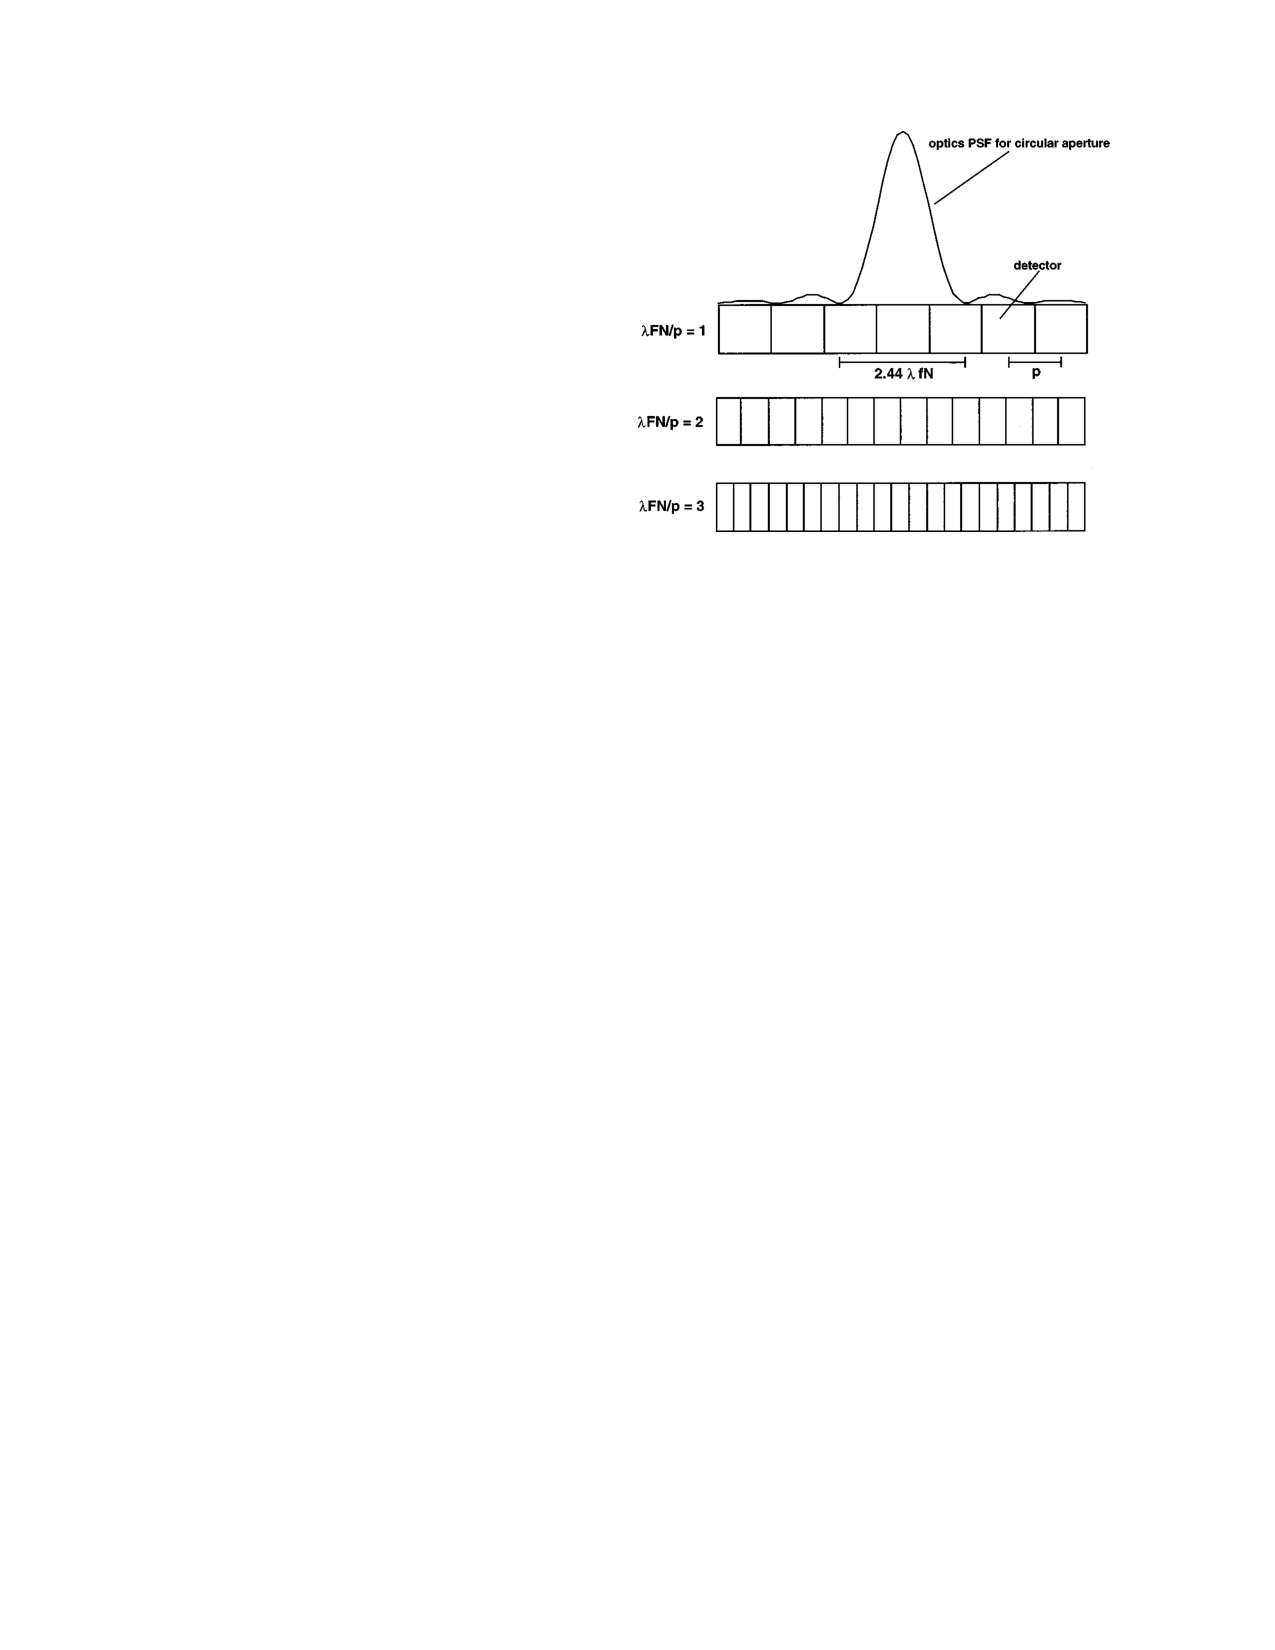
\includegraphics[width=0.42\textwidth]{figures/Q_fiete.pdf}
% \caption{Spatial interpretation of Q sampling a diffraction-limited PSF.  Adapted from \cite{fiete_q})}
% \end{figure} 

Beyond a statement of the Nyquist criterion, $Q$ is a very useful parameter by which to evaluate and compare systems.  For more see \cite{fiete_q}.  

\subsection{Photon Radiometry}

In order to not have to carry full radiometry for every calculation, we will define a payload photo-electron gain, 

\begin{equation}
k_{pe} \equiv \frac{\dot{N}_{e^-}^{std}}{L}
\label{eq:k_pe}
\end{equation}

Where 

\begin{equation*}
    L = \int_{\lambda_1}^{\lambda_2}L_{\lambda}(\lambda)d\lambda
\end{equation*}

is radiance at aperture in W/m$^2$-sr, $QE$ is quantum efficiency, $\Delta \lambda$ is spectral bandwidth and $\dot{N}_{e^-}^{std}$ is photo-electron generation rate for the case of $QE=1$, $Q=1$.

Moving forward, we will use $k_{pe} = 2\times 10^5$ e$^-$-sr-um-m$^2$/J\footnote{Given $\Delta \lambda = 0.5$um, $L = 100$ W/m$^2$-sr-um, this equates to $\dot{N}_{e^-}^{std} = 1\times 10^7$ e$^-$ / s or 5,000 photo-electrons accumulated in a 1ms integration time on a $Q=1$, $QE=0.5$ system}

Now we have a simple relationship useful in comparing systems radiometrically:

\begin{equation}
\dot{N}_{e^-} = \frac{k_{pe} L \times QE}{Q^2}
\label{eq:N_e_dot}
\end{equation}

Typically remote sensing systems report signal to noise at a radiance a small fraction of the saturation radiance.  We will define this ratio of typical to saturation radiance - 

\begin{equation}
\alpha = \frac{L_{typ}}{L_{sat}}
\label{eq:alpha}
\end{equation}

For systems in which shot and read noise dominate
\begin{equation}
SNR = \frac{s}{\sigma_{rd} + \sqrt{s}}
\label{eq:snr}
\end{equation}

where $s$ is the signal magnitude in photoelectrons and $\sigma_{rd}$ is read noise in RMS photoelectrons.

Finally, we come to a very useful relationship for a single exposure in eq. \eqref{eq:s} -
\begin{equation}
s = \alpha k_{pe}L_{sat} \frac{t_{int}QE}{Q^2}
\label{eq:s}
\end{equation}

Note that in several of the modalities, digital over-sampling is utilized.  In that case, the effective output signal level for a ground sample is 
\begin{equation*}
    s^{eff} = N_s s
\end{equation*}

where $N_s$ is the oversampling ratio.

\onecolumn
\section{Appendix B: Sensor Table}
\label{sec:appendix_b}

\begin{table}[t]
\centering
\resizebox{0.96 \linewidth}{!}{%
\begin{tabular}{cccccccccc}
\toprule
\textbf{Model} & \textbf{Type} & \textbf{Shutter} & \textbf{Width} 
& \textbf{Height} & \textbf{FPS} & \textbf{Pixel Size (um)} & 
\textbf{QE (525 nm)} & \textbf{$N_{rd}$}  & \textbf{$N_{e^-}^{FWC}$} \\ 

\midrule 
                        
Sony ICX424 & CCD & Global & 648 & 488 & 84 & 7.4 & 46 & 12.9 & 13932\\ 
Sony ICX424 & CCD & Global & 648 & 488 & 84 & 7.4 & 53 & 12.0 & 13701\\ 
Sony ICX414 & CCD & Global & 648 & 488 & 90 & 9.9 & 39 & 19.4 & 25949\\ 
Sony ICX618 & CCD & Global & 648 & 488 & 120 & 5.6 & 70 & 11.7 & 14508\\ 
Sony ICX693 & CCD & Global & 808 & 608 & 50 & 6.0 & 71 & 11.2 & 20024\\ 
Sony ICX204 & CCD & Global & 1032 & 776 & 31 & 4.7 & 42 & 12.1 & 11944\\ 
Sony ICX692 & CCD & Global & 1288 & 728 & 30 & 4.1 & 72 & 8.6 & 11551\\ 
Sony ICX445 & CCD & Global & 1288 & 964 & 30 & 3.8 & 62 & 10.3 & 9686\\ 
Sony ICX445 & CCD & Global & 1288 & 964 & 30 & 3.8 & 66 & 9.2 & 9196\\ 
Sharp RJ33J4CA3DE & CCD & Global & 1288 & 964 & 30 & 3.8 & 70 & 5.4 & 7384\\ 
Sony ICX445 & CCD & Global & 1288 & 964 & 30 & 3.8 & 68 & 10.1 & 9231\\ 
Sony ICX445 & CCD & Global & 1288 & 964 & 31 & 3.8 & 61 & 7.6 & 7347\\ 
Sony ICX267 & CCD & Global & 1384 & 1032 & 18 & 4.7 & 53 & 11.5 & 10366\\ 
Sony ICX825 & CCD & Global & 1384 & 1032 & 45 & 6.5 & 73 & 8.3 & 22856\\ 
Sony ICX285 & CCD & Global & 1384 & 1036 & 30 & 6.5 & 56 & 11.9 & 16408\\ 
Sony ICX274 & CCD & Global & 1624 & 1224 & 15 & 4.4 & 59 & 8.3 & 7969\\ 
Sony ICX674 & CCD & Global & 1920 & 1440 & 26 & 4.5 & 67 & 9.4 & 14693\\ 
Sony ICX818 & CCD & Global & 1928 & 1448 & 13 & 3.7 & 76 & 10.5 & 10936\\ 
Sony ICX687 & CCD & Global & 1928 & 1448 & 15 & 3.7 & 79 & 9.7 & 11586\\ 
Sony ICX687 & CCD & Global & 1928 & 1448 & 26 & 3.7 & 68 & 10.2 & 9039\\ 
Sony ICX808 & CCD & Global & 2024 & 2024 & 18 & 3.1 & 75 & 9.3 & 6459\\ 
Sony ICX655 & CCD & Global & 2448 & 2048 & 8 & 3.5 & 60 & 9.4 & 5856\\ 
Sony ICX625 & CCD & Global & 2448 & 2048 & 15 & 3.5 & 58 & 8.7 & 6168\\ 
Sony ICX625 & CCD & Global & 2448 & 2048 & 15 & 3.5 & 57 & 8.2 & 5903\\ 
Sharp RJ32S4AA0DT & CCD & Global & 2448 & 2048 & 7 & 3.5 & 57 & 5.5 & 8086\\ 
Sony ICX694 & CCD & Global & 2736 & 2192 & 13 & 4.5 & 73 & 10.5 & 14446\\ 
Sony ICX694 & CCD & Global & 2736 & 2192 & 25 & 4.5 & 74 & 10.9 & 14227\\ 
Sony ICX694 & CCD & Global & 2736 & 2192 & 13 & 4.5 & 72 & 10.9 & 14959\\ 
Sony ICX814 & CCD & Global & 3376 & 2704 & 9 & 3.7 & 75 & 9.4 & 9996\\ 
Sony ICX834 & CCD & Global & 4240 & 2824 & 7 & 3.1 & 78 & 10.9 & 6125\\ 
Kodak KAI-29050 & CCD & Global & 6576 & 4384 & 4 & 5.5 & 43 & 12.0 & 20000\\ 
Kodak KAI-47051 & CCD & Global & 8856 & 5280 & 7 & 5.5 & 43 & 10.0 & 20000\\ 
On Semi KAF-50100 & CCD & Global & 8176 & 6132 & 1 & 6.0 & 62 & 12.5 & 40000\\ 
Aptina AR0134 & CMOS & Global & 1280 & 960 & 52 & 3.8 & 77 & 6.6 & 5542\\ 
e2v EV76C560 & CMOS & Global & 1280 & 1024 & 60 & 5.3 & 59 & 25.1 & 8384\\ 
e2v EV76C560 & CMOS & Global & 1280 & 1024 & 60 & 5.3 & 61 & 25.3 & 7506\\ 
ON Semi VITA1300 & CMOS & Global & 1280 & 1024 & 150 & 4.8 & 61 & 26.3 & 10226\\ 
ON Semi PYTHON 1300 & CMOS & Global & 1280 & 1024 & 149 & 4.8 & 59 & 9.3 & 6057\\ 
ON Semi PYTHON 1300 & CMOS & Global & 1280 & 1024 & 170 & 4.8 & 59 & 9.2 & 5779\\ 
Sony IMX035 & CMOS & Rolling & 1328 & 1048 & 120 & 3.6 & 77 & 6.0 & 15491\\ 
e2v EV76C570 & CMOS & Global & 1600 & 1200 & 60 & 4.5 & 66 & 24.2 & 7788\\ 
Sony IMX174 & CMOS & Global & 1920 & 1200 & 162 & 5.9 & 76 & 6.8 & 32513\\ 
Sony IMX249 & CMOS & Global & 1920 & 1200 & 41 & 5.9 & 80 & 7.1 & 33105\\ 
Sony IMX252 & CMOS & Global & 2038 & 1536 & 121 & 3.5 & 76 & 2.3 & 10482\\ 
Sony IMX265 & CMOS & Global & 2048 & 1536 & 55 & 3.5 & 71 & 2.9 & 9777\\ 
CMOSIS CMV4000 & CMOS & Global & 2048 & 2048 & 90 & 5.5 & 53 & 16.8 & 7620\\ 
Sony IMX264 & CMOS & Global & 2448 & 2048 & 35 & 3.5 & 69 & 2.3 & 9869\\ 
Sony IMX250 & CMOS & Global & 2448 & 2048 & 75 & 3.5 & 76 & 2.4 & 10361\\ 
Aptina MT9P031 & CMOS & Rolling & 2592 & 1944 & 13 & 2.2 & 63 & 7.6 & 6693\\ 
Sony IMX255 & CMOS & Global & 4096 & 2160 & 43 & 3.5 & 71 & 2.4 & 10435\\ 
Sony IMX253 & CMOS & Global & 4096 & 3000 & 30 & 3.5 & 72 & 2.4 & 10563\\ 
Sony IMX342 & CMOS & Global & 6464 & 4852 & 35 & 3.5 & 72 & 2.4 & 10500\\ 
Sony IMX367 & CMOS & Global & 4416 & 4428 & 43 & 3.5 & 72 & 2.4 & 10500\\ 
BAE CIS2521 & CMOS & Global & 2560 & 2160 & 50 & 6.5 & 55 & 5.0 & 30000\\ 
BAE LTN4625a & CMOS & Global & 4608 & 2592 & 120 & 5.5 & 55 & 5.0 & 40000\\ 
On Semi Python 25k & CMOS & Global & 5120 & 5120 & 80 & 4.5 & 50 & 14.0 & 12000\\ 
CMOSIS CMV12000 & CMOS & Global & 4096 & 3072 & 132 & 5.5 & 45 & 12.5 & 13000\\ 
CMOSIS CMV20000 & CMOS & Global & 5120 & 3840 & 30 & 6.5 & 45 & 8.0 & 15000\\ 
CMOSIS CMV50000 & CMOS & Global & 7920 & 6004 & 30 & 4.6 & 45 & 8.8 & 14500\\ 
Sony A7R & CMOS & Rolling & 7392 & 4920 & 5 & 4.9 & 50 & 4.3 & 49000\\ 
GPIXEL 3005 & CMOS & Rolling & 30000 & 5000 & 10 & 5.5 & 50 & 3.9 & 23000\\ 
GPIXEL 1205 & CMOS & Rolling & 12000 & 5000 & 10 & 5.5 & 50 & 2.9 & 22000\\ 
GSENSE 5130 & CMOS & Global & 5056 & 2968 & 67 & 4.2 & 50 & 5.0 & 16000\\ 

\end{tabular}%
}
\caption{All sensors considered in analyses}
\label{table:all_sensors}
\end{table}


\twocolumn

\bibliography{IEEEabrv,main}

\end{document}
